\documentclass[12pt,a4paper]{report}

%\includeonly{cover/cimlap, chapters/1_introduction}

\usepackage{styles/dolgozat}

% programkód beillesztéséhez
\usepackage{listings}
% listing float neve
\renewcommand{\lstlistingname}{Programkód}
%\renewcommand{\lstlistlistingname}{Programkódok listája}
%saját listings style-ok, és a style-t használó parancsok definíciói
\usepackage{styles/cpp}
\usepackage{styles/python}
%\usepackage{styles/java}
%\usepackage{styles/rust}

%% egyéb csomagok betöltése itt, vagy a dolgozat.sty fájlban

\usepackage{hyperref}
% cleveref csomag és beállításai -- az egyetlen, amit a hyperref után kell betölteni!
\usepackage{styles/refs}

\begin{document}

\pagestyle{empty}
\pagenumbering{gobble}

\begin{titlepage}
\centering
% A Miskolci Egyetem címere
\vspace*{2cm}
\huge\textsc{\textbf{Szakdolgozat}}\\[1cm]
%\vspace*{1cm}

\includegraphics[width=4.8cm, height=4cm,keepaspectratio]{images/me_logo.png}\\
\textbf{\textsc{Miskolci Egyetem}}

\vspace*{2cm}

% A szakdolgozat címe, akár több sorban is
{\LARGE\textbf{Az én szakdolgozatom}}

\vspace*{2cm}
% A hallgató neve, évfolyam, szak(ok), a konzulens(ek) neve
\large
\textbf{Készítette:}\\[0.8ex]
Szendrei Gábor\\[0.8ex]
Programtervező informatikus

\vspace*{0.5cm}
\textbf{Témavezető:}\\[0.8ex]
Dr.\ Vadon Viktória

\vfill

% Keltezés: Hely, év
\large
\textbf{\textsc{Miskolc, 2023}}

\end{titlepage}
%Feladatkiiras
\noindent
\textsc{\textbf{Miskolci Egyetem}}\\
Gépészmérnöki és Informatikai Kar\\
Alkalmazott Matematikai Intézeti Tanszék\hspace*{4cm}\hfil \textbf{Szám:}

\vspace{0.5cm}
\begin{center}
\large\textsc{\textbf{Szakdolgozat Feladat}}
\end{center}
\vspace{0.5cm}

Szendrei Gábor (V9ZK10) programtervező informatikus jelölt részére.

\bigskip
\noindent\textbf{A szakdolgozat tárgyköre:} kulcsszavak, hasonlók

\bigskip
\noindent\textbf{A szakdolgozat címe:} A dolgozat címe

\bigskip
\noindent\textbf{A feladat részletezése:}

\medskip

\emph{Ide kell a feladatkiírásban szereplő szöveget betenni.}

\medskip

\emph{(Kisebb tagolás lehet benne, hogy jól nézzen ki.)}

\vfill

\noindent\textbf{Témavezető:} Témavezető neve (beosztása)

% \noindent\textbf{Konzulens(ek):} (akkor kötelezõ, ha a témavezetõ nem valamelyik matematikai tanszékrõl való; de persze lehet egyébként is)\newline

\bigskip
\noindent\textbf{A feladat kiadásának ideje:}

%\noindent\textbf{A feladat beadásának határideje:}

\vspace{1.5cm}

\hfill\makebox[6cm]{\dotfill}

\hfill\makebox[6cm]{szakfelelős}

\clearpage

\vspace*{1cm}  
\begin{center}
\large\textsc{\textbf{Eredetiségi Nyilatkozat}}
\end{center}
\vspace*{2cm}  

Alulírott \textbf{Szendrei Gábor}; Neptun-kód: \texttt{V9ZK10} a Miskolci Egyetem Gépészmérnöki és Informatikai Karának végzős Programtervező informatikus szakos hallgatója ezennel büntetőjogi és fegyelmi felelősségem tudatában nyilatkozom és aláírásommal igazolom, hogy \textit{Szakdolgozat Címe}
című szakdolgozatom saját, önálló munkám; az abban hivatkozott szakirodalom
felhasználása a forráskezelés szabályai szerint történt.

\medskip
Tudomásul veszem, hogy szakdolgozat esetén plágiumnak számít:
\begin{itemize}
\item szószerinti idézet közlése idézőjel és hivatkozás megjelölése nélkül;
\item tartalmi idézet hivatkozás megjelölése nélkül;
\item más publikált gondolatainak saját gondolatként való feltüntetése.
\end{itemize}

Alulírott kijelentem, hogy a plágium fogalmát megismertem, és tudomásul veszem, hogy
plágium esetén szakdolgozatom visszautasításra kerül.

\vspace*{3cm}

\noindent Miskolc, \makebox[2cm]{\dotfill}. év \makebox[2cm]{\dotfill}. hó \makebox[2cm]{\dotfill}. nap

\vspace*{3cm}

\hfill\makebox[6cm]{\dotfill}

\hfill\makebox[6cm]{Hallgató}



\clearpage

\newcommand{\ki}{témavezető(k)}
\newsavebox{\alairas}
\begin{lrbox}{\alairas}
\begin{tabular}{c@{\hspace{2cm}}c}
\makebox[4cm]{\dotfill} & \makebox[5cm]{\dotfill} \\
dátum & \ki \\
\end{tabular}
\end{lrbox}
\newcommand{\dotline}{\makebox[5cm]{\dotfill}}
\newcommand{\shortdotline}{\makebox[3.5cm]{\dotfill}}

\noindent 1.
\begin{tabular}[t]{cl}
\multirow{2}{*}{A szakdolgozat feladat módosítása}
&szükséges (módosítás külön lapon) \\
& nem szükséges\\[1ex]
\end{tabular}

\begin{center}
\usebox{\alairas}
\end{center}

\smallskip

\noindent 2. A feladat kidolgozását ellenőriztem:

\begin{center}
\begin{tabular}{c@{\hspace*{2cm}}c}
témavezető (dátum, aláírás): & konzulens (dátum, aláírás):\\
\dotline & \dotline \\
\dotline & \dotline \\
\dotline & \dotline 
\end{tabular}
\end{center}

\smallskip

\noindent 3. A szakdolgozat beadható:

\begin{center}
\usebox{\alairas}
\end{center}

\noindent 4.
\begin{tabular}[t]{@{}l@{\hspace*{1mm}}l@{\hspace*{1mm}}l}
A szakdolgozat & \shortdotline & szövegoldalt\\
              & \shortdotline & program protokollt (listát, felhasználói leírást)\\
              & \shortdotline & elektronikus adathordozót (részletezve)\\
              & \shortdotline \\
              & \shortdotline & egyéb mellékletet (részletezve)\\
              & \shortdotline 
\end{tabular}
\newline tartalmaz.

\begin{center}
\usebox{\alairas}
\end{center}

\noindent 5.
\begin{tabular}[t]{ll}
\multirow{2}{*}{A szakdolgozat bírálatra} & bocsátható\\
& nem bocsátható\\
\end{tabular}

\smallskip

\noindent A bíráló neve: \makebox[8cm]{\dotfill}

\renewcommand{\ki}{szakfelelős}
\begin{center}
\begin{tabular}{c@{\hspace{2cm}}c}
\makebox[4cm]{\dotfill} & \makebox[5cm]{\dotfill} \\
dátum & \ki \\
\end{tabular}
\end{center}

\noindent 6.
\begin{tabular}[t]{lll}
A szakdolgozat osztályzata \\
& a témavezető javaslata: & \makebox[2.5cm]{\dotfill} \\
& a bíráló javaslata: & \makebox[2.5cm]{\dotfill} \\
& a szakdolgozat végleges eredménye: & \makebox[2.5cm]{\dotfill}
\end{tabular}

\bigskip\bigskip

\noindent Miskolc, \makebox[4cm]{\dotfill} \hfill \makebox[8cm]{\dotfill} 

\hfill \makebox[8cm]{a Záróvizsga Bizottság Elnöke} 


\tableofcontents

\clearpage
\pagenumbering{arabic}
\pagestyle{fancy}

\chapter{Bevezetés}

A fejezet célja, hogy a feladatkiírásnál kicsit részletesebben bemutassa, hogy miről fog szólni a dolgozat.
Érdemes azt részletezni benne, hogy milyen aktuális, érdekes és nehéz probléma megoldására vállalkozik a dolgozat.

Ez egy egy-két oldalas leírás.
Nem kellenek bele külön szakaszok (section-ök).
Az irodalmi háttérbe, a probléma részleteibe csak a következő fejezetben kell belemenni.
Itt az olvasó kedvét kell meghozni a dolgozat többi részéhez.

\chapter{Játékfejlesztés és a Pygame}

\section{Bevezetés a Játékfejlesztés Világába}

\indent \indent A játékfejlesztés a modern szórakoztatóipar egyik legszerteágazóbb és izgalmasabb területe, amely számtalan lehetőséget rejt magában a kreativitás kibontakoztatására és az élmények megteremtésére. Ennek a fejezetnek az elején bemutatom, hogy mit jelent játékot fejleszteni, milyen kihívásokkal jár, és milyen lehetőségeket kínál.

\subsection{Mit jelent játékot fejleszteni?}
\indent \indent Játékot fejleszteni egy olyan folyamat, amely során valamilyen virtuális alkalmazást tervezünk, készítünk és tesztelünk. Ezek a játékok szórakoztatnak, kihívások elé állítanak, vagy éppen történeteket mesélnek el a játékosoknak. A játékfejlesztés során számos különböző területet érintünk, mint például a grafika, a hang, a programozás, a játéktervezés és a narratíva.

A játékfejlesztés során a következő elemeket kell figyelembe venni:

\begin{itemize}
    \item Játéktervezés: A játékmechanizmusok, pályatervezés, karakterek és sztori kidolgozása.
    \item Grafika és dizájn: A játékvilág megtervezése, karakterek és tájak kinézetének megalkotása.
    \item Hang és zene: A játékhangulat meghatározása zenei és hanghatásokkal.
    \item Programozás: A játék mechanizmusainak és logikájának implementálása.
\end{itemize}
\subsection{A játékfejlesztés kihívásai és lehetőségei}
\indent \indent A játékfejlesztés izgalmas, de komplex folyamat, amely számos kihívást rejt magában:

Technikai kihívások: A játékfejlesztéshez fejlett szoftveres és hardveres ismeretekre van szükség. A játék motorok, programozási nyelvek, és grafikai eszközök használata összetett feladatokkal jár.

Kreativitás: A jó játékok egyediséget és kreativitást követelnek meg a játéktervezőktől. Az új és izgalmas játékmechanizmusok kitalálása kulcsfontosságú.

Projektmenedzsment: A játékfejlesztés projektek hosszú és komplex folyamatok, amelyek határidőket és költségvetéseket igényelnek. A megfelelő projektmenedzsment kritikus fontosságú.

Felhasználói élmény: A játékosok elégedettségének és élvezetének biztosítása kiemelten fontos. A játéktervezés és felhasználói felület optimalizálása elengedhetetlen.

Ugyanakkor a játékfejlesztésben óriási lehetőségek rejlenek:

Kreatív kibontakozás: A játékfejlesztés lehetőséget ad a kreativitás megnyilvánulására, ahol csak a képzelet szab határt.

Közösség és verseny: A játékfejlesztők részt vehetnek aktív közösségekben, és akár versenyeken is, ahol megmutathatják tehetségüket és fejlődésüket.

Szórakoztatás: A jó játékok milliók számára jelentenek kikapcsolódást és szórakozást, és hűséges rajongótábort hozhatnak létre.


\section{Játékfejlesztő Könyvtárak és Eszközök}

\indent \indent A játékfejlesztéshez elérhető könyvtárak és eszközök rendkívül fontosak a fejlesztők számára, hiszen segítenek a játékok fejlesztésében és optimalizálásában. Ebben a részben áttekintünk néhány közismert könyvtárat és eszközt, amelyeket játékfejlesztéshez használnak.

\subsection{Unity: A 3D játékfejlesztés platformja}\cite{unity-doc}
\indent \indent A Unity a játékfejlesztők körében rendkívül népszerű, mivel egyszerűen kezelhető és széles körű lehetőségeket kínál a játékok létrehozásához. A platform komplex fejlesztői eszközökkel rendelkezik, például szkriptelési lehetőségekkel és beépített folyamatkezelővel, amelyek megkönnyítik a játékfejlesztést.

A Unity támogatja a 2D és 3D játékok készítését egyaránt, így a fejlesztők szabadon választhatják meg a stílust és a műfajt. A platform lehetővé teszi a cross-platform fejlesztést, amely azt jelenti, hogy egyetlen projektből készíthetünk játékokat különböző platformokra, például Windows, iOS, Android vagy konzolokra.

A Unity erős grafikai motorokkal rendelkezik, amelyek lehetővé teszik a gyönyörű és részletes grafikák létrehozását. Emellett fizikai motorjai valósághű mozgást és ütközéseket biztosítanak, ami a játékélményt még valóságosabbá teszi.

A folyamatos támogatás és a nagy közösség miatt A Unity egy kiváló választás a játékfejlesztők számára, akik minőségi játékokat szeretnének létrehozni a különböző platformokon. A Unity segítségével a fejlesztők könnyen hozzáférhetnek az új funkciókhoz és frissítésekhez, hogy folyamatosan fejleszthessék játékaikat.
\subsection{Java: Népszerű választás játékfejlesztők számára}\cite{java-doc}
\indent \indent A Java egy platformfüggetlen, objektumorientált programozási nyelv, amelyet a játékfejlesztésben is széles körben alkalmaznak, különösen az Android platformon. A Java játékok fejlesztéséhez különféle fejlesztői eszközök és könyvtárak állnak rendelkezésre.

Például, a Java játékok fejlesztéséhez számos integrált fejlesztői környezet (IDE) érhető el, mint például az Android Studio vagy a Eclipse, amelyek segítenek a játékok tervezésében és kódolásában. Ezek az IDE-k számos hasznos eszközt és szolgáltatást kínálnak a fejlesztőknek, például hibakeresőt és kódszerkesztőt.

A Java játékok grafikai részének fejlesztéséhez számos grafikai könyvtár is rendelkezésre áll, például a LibGDX vagy a JavaFX. Ezek a könyvtárak lehetővé teszik a játékgrafikák létrehozását, animációk kezelését és a felhasználói felület kialakítását.

Emellett a Java egy erős közösséggel rendelkezik, ami azt jelenti, hogy a fejlesztők könnyen hozzáférhetnek különböző fejlesztői eszközökhöz és könyvtárakhoz, amelyek segítik a játékfejlesztést. Példaként említhetők a játékfejlesztéshez használt függvénykönyvtárak, például a LWJGL (Lightweight Java Game Library), amely lehetővé teszi a háromdimenziós játékok fejlesztését Java nyelven.
\subsection{C\#: Kiemelt szerepű programozási nyelv a játékfejlesztők körében}\cite{csharp-doc}

\indent \indent A C\# egy modern, objektumorientált programozási nyelv, melyet széles körben alkalmaznak a játékfejlesztés területén, különösen A Unity játékmotorral. A Unity egyike a legnépszerűbb játékfejlesztő platformoknak, és C\#-t használ a játéklogika és szkriptelés megvalósításához, így lehetővé téve a fejlesztők számára a cross-platform játékok készítését.

A C\# rendelkezik egy erős és fejlett fejlesztői környezettel, amely segíti a fejlesztőket a játéktervezésben és kódolásban. Az integrált fejlesztői eszközök, például a Visual Studio, hatékony eszközöket nyújtanak a kódírás, hibakeresés és teljesítményoptimalizálás terén.

A Unity és C\# együttes használata lehetővé teszi a fejlesztők számára a könnyű és hatékony játékfejlesztést számos platformra, mint például számítógépek, mobil eszközök és konzolok. Ez a kombináció erős grafikai motorokkal, fizikai motorokkal és egyéb eszközökkel is rendelkezik, amelyek segítik a játékélmény kialakítását és optimalizálását.

Mivel a C\# egy népszerű és jól támogatott nyelv a játékfejlesztésben, a fejlesztők könnyen hozzáférhetnek különböző fejlesztői eszközökhöz és könyvtárakhoz, amelyek elősegítik a játékfejlesztést és a játéktervezést.
\subsection{C++: A régebbi játékok elengedhetetlen nyelve}\cite{cpp-doc}

\indent \indent A C++ egy erőteljes és hatékony programozási nyelv, amely gyakran előfordul a játékfejlesztés világában, különösen a nagy teljesítményű játékok és konzolplatformok esetében. A C++ nyelv lehetővé teszi a fejlesztők számára, hogy közvetlenül a hardverre programozzanak, ami rendkívül nagy szabadságot és teljesítményt nyújt.

A játékfejlesztők körében a C++ kiemelkedően kedvelt nyelv, mivel lehetőséget nyújt a nagy teljesítményű játékok létrehozására és a hardverrel való közvetlen kapcsolat kialakítására. Számos játékfejlesztő könyvtár és motor támogatja a C++ nyelvet, amelyek segítik a játékfejlesztőket a projektjeik gyorsabb és hatékonyabb megvalósításában.

Az eszközök és nyelvek kiválasztása a projekt specifikus igényektől és a fejlesztői készségektől függ. Fontos megérteni, hogy minden eszköznek és nyelvnek megvannak a saját előnyei és korlátai, és ezeket a projekt céljaival és a fejlesztőcsapat készségeivel kell összeegyeztetni annak érdekében, hogy a lehető legjobb játékélményt nyújtsák a játékosoknak.


\section{Python a játékfejlesztésben}

\indent \indent A Python egy kiválóan használható programozási nyelv a játékfejlesztéshez, és sok előnnyel rendelkezik a fejlesztők és a játéktervezők számára. Ebben a fejezetben kifejtem, miért érdemes Pythonnal dolgozni játékok tervezésekor, és milyen alapvető tulajdonságok és lehetőségek teszik ezt a nyelvet vonzóvá a játékfejlesztés világában.

\subsection{Miért jó a Python?}\cite{why-is-python}
\indent \indent Olvashatóság és Egyszerűség:
Python kódot írni könnyű és gyors. A Python nyelv szintaxisa rendkívül olvasható és hasonlít az angol nyelvre, ami megkönnyíti a kód értelmezését. A könnyű olvashatóság a fejlesztési időt csökkentheti és csökkentheti a hibák számát.

Gyors Fejlesztés:
Lehetővé teszi a gyors prototípusok létrehozását. A gyors prototípusok segítenek a játék ötleteinek gyors validálásában és tesztelésében, mielőtt hosszú fejlesztési ciklusokba kezdünk.

Széles Közösség és Támogatás:
Rendelkezik egy nagy és elkötelezett fejlesztői közösséggel, ami számos kiegészítő könyvtárat és eszközt kínál a játékfejlesztőknek. Ez a közösség folyamatosan fejleszti és frissíti a nyelvet és az eszközöket.


\subsection{A Python és a Játékfejlesztés}\cite{python-in-game-dev}
\indent \indent A Python programozási nyelvet egyre gyakrabban alkalmazzák a játékfejlesztés területén. Bár eredetileg nem a legnépszerűbb választás volt ebben a szektorban, az utóbbi években számos előnye miatt kezdett teret hódítani.

A Python játékfejlesztésre való áttérést elősegíti az egyszerűsége és olvashatósága, amely lehetővé teszi a fejlesztők számára, hogy a játékmechanizmusokra és a játékélményre összpontosítsanak, anélkül hogy túlzottan mélyen kellene merülniük a technikai részletekbe.

Ezenkívül a Python platformfüggetlen, így a fejlesztők könnyedén exportálhatják játékaikat különböző rendszerekre, például Windows, macOS vagy Linux alá, ami tovább növeli a nyelv vonzerejét a játékfejlesztők számára.

Mivel a Python játékfejlesztés területén egyre népszerűbbé válik, egyre több játék fejlesztése zajlik ezen a platformon, és továbbra is új lehetőségek és fejlesztői eszközök válnak elérhetővé a játékfejlesztők számára.

\section{Pygame}\cite{pygame}
\indent \indent A Pygame egy nyílt forráskódú programozási platform és könyvtár, mely lehetővé teszi játékok és multimédiás alkalmazások fejlesztését a Python programozási nyelv segítségével. Különösen népszerű a játékfejlesztők körében, mivel könnyen használható és rendkívül rugalmas. A Pygame rétegekben épül fel, amelyek lehetővé teszik a felhasználók számára, hogy kezeljék az ablakokat, az eseményeket, a grafikát és a hangot.
\subsection{Pygame lehetőségei}
\indent \indent A Pygame rendkívül sokoldalú eszközöket és lehetőségeket kínál a játékfejlesztők számára:

Grafikai megjelenítés: Lehetővé teszi a grafikus elemek létrehozását és kezelését, beleértve a felületeket, háttérképeket és megjelenítési funkciókat is.

Hangkezelés: A könyvtár lehetővé teszi hangfájlok lejátszását, hanghatások és zene hozzáadását a játékhoz.

Inputkezelés: Segítségével könnyedén kezelhetők a felhasználói inputok, például a billentyűzet és egér események.

Multiplatform támogatás: Rendkívül hordozható, és szinte minden platformon és operációs rendszeren fut, beleértve Linuxot, Windowst, MacOS-t és másokat.

Hordozhatóság: Alkalmazható számos eszközön és operációs rendszeren, beleértve a kézi eszközöket, játékkonzolokat és a One Laptop Per Child (OLPC) számítógépét is.

Egyszerűség: Könnyen megtanulható és használható, és kiválóan alkalmas fiatalabb és idősebb játékfejlesztők számára egyaránt.

Modularitás: Lehetőséget ad arra, hogy a különböző modulokat külön-külön inicializálja és használja, így testreszabhatja a fejlesztést az igényeinek megfelelően.



\subsection{Pygamemel Készített Sikeres Játékok}
\indent \indent A Pygame egy olyan eszköz, amely lehetővé teszi a fejlesztők számára, hogy kreatív és sokoldalú játékokat hozzanak létre. Néhány példa sikeres Pygame projektekre:

\begin{itemize}

    \item Cave Story (2004): Egy kalandjáték, amelyet Daisuke Amaya készített. A játék nagy sikert aratott a játékosok körében, és azóta is népszerű maradt. \cite{CaveStory}
    \item Super Meat Boy (2010): Egy gyors tempójú platformjáték, amelyben a játékos egy húsból készült fiút irányít, aki megpróbál eljutni egy másik húsból készült lányhoz.\cite{SuperMeatBoy}
    \item Braid (2008): Egy különleges platformjáték, amelyben a játékosnak időutazást kell alkalmaznia a játék különböző szintjein.\cite{Braid}
\end{itemize}


\subsection{Prototípusok és koncepciók}
\indent \indent A pygame lehetővé teszi prototípusok készítését és koncepciók tesztelését a valóságban. A prototípusok és koncepciók tesztelése segíthet a fejlesztőknek abban, hogy javítsák a játékaikat, mielőtt azok nagyszabású fejlesztésbe kerülnek. A pygamet gyakran használják új játékmechanikák, játékstílusok tesztelésére, mivel gyorsan és hatékonyan lehet vele prototípusokat készíteni.

\subsection{További tudnivalók a Pygame-ről}

\indent \indent Széleskörű Közösség és Források:
A Pygame hatalmas fejlesztői közösséggel rendelkezik, ami azt jelenti, hogy rengeteg dokumentáció, tutorial és fórum áll rendelkezésre a segítségnyújtáshoz és a problémamegoldáshoz. Az aktív közösség folyamatosan fejleszti és frissíti a Pygame-et, így a fejlesztők mindig naprakész forrásokhoz férhetnek hozzá.

Könnyen Tanulható:
A Pygame olyan egyszerűen használható, hogy akár gyerekek és fiatalabb játékfejlesztők is könnyen megtanulhatják a használatát. A kezdeti lépések után a fejlesztők gyorsan építhetnek fel játékokat és alkalmazásokat a Pygame segítségével.


\subsection{Összegzés}
\indent \indent A Pygame és hasonló játékfejlesztő eszközök széles körű alkalmazást kínálnak a modern társadalomban.
 Ezek az eszközök nem csupán játékok készítésére használhatók, hanem hatékony eszközök a tanulás,
  a kutatás és a kreativitás terén is. A játékosított tanulás révén motiválóbbá tehetjük az oktatást, 
  míg a kognitív kutatásban lehetőséget nyújtanak az emberi kogníció tanulmányozására.
   Emellett a játékfejlesztés lehetőséget ad az ötletelésre és a kreatív kifejezésre is.
    Bármilyen szinten is legyen valakinek a játékfejlesztés terén,
 a Pygame és hasonló eszközök segítségével saját projekteket hozhat létre és járulhat hozzá
  a tudásunk bővítéséhez és a különböző területeken való alkalmazásukhoz.
   A játékok nagyon hasznos eszközök, amelyeket a gyerekek és felnőttek is élveznek.
    Rengeteg hasznos készséget lehet elsajátítani játszás során, ez a számítógépes játékokkal sincsen másképp.
A kreatív és kihívást kedvelő embereknek a játékfejlesztés egy kiváló lehetőség arra,
 hogy kipróbálják magukat és megmutassák kreativitásukat.
  A játékfejlesztés során a fejlesztők számos készséget elsajátíthatnak, például a programozást,
a dizájnt és a projektmenedzsmentet. A játékfejlesztés egyre népszerűbb a modern társadalomban,
 és egyre több ember kezd el játszani, ezért a fejlesztőkre is igen nagy az igény. 
 Ez a fajta munka rengeteg lehetőséget kínál a kreativitás kibontakoztatására és a tanulás és fejlődés terén.
  A jövőben is szükség lesz a játékfejlesztésben jártas emberekre, hiszen ez örökké velünk
   fog maradni valamilyen formában.


\section{Pygame és Ren'Py Összehasonlítása} \cite{pygame-renpy}
\indent \indent A Pygame és a Ren'Py két olyan kiváló szoftverkönyvtár, amelyeket a játékfejlesztők és vizuális novellák készítői használnak világszerte. Bár első pillantásra talán nincsenek sok közös vonásuk, mindkét platform a játékok és interaktív történetek fejlesztésére szolgál, és számos hasonlóság és különbség rejlik bennük. Ebben a fejezetben részletesen megvizsgáljuk a Pygame és a Ren'Py funkcióit, lehetőségeit, valamint az alkalmazásukat különböző projektekhez. Ezzel a közvetlen összehasonlítással lehetőséget teremtünk arra, hogy megtudjuk, melyik könyvtár a legalkalmasabb az adott célkitűzések és projektek szempontjából, és milyen előnyökkel és korlátozásokkal jár az alkalmazásuk.

\subsection{Felhasználási terület}
\indent \indent A Pygame és a Ren'Py két különböző, de rendkívül hasznos eszköz a játékfejlesztők és vizuális novellák alkotói számára. A Pygame sokoldalúságának köszönhetően szinte bármilyen típusú játékfejlesztésre alkalmazható, így lehetőséget biztosít akció-játékok, platformjátékok, vagy éppen puzzle-játékok létrehozására. Azonban a Ren'Py specifikus specializációja a szövegalapú vizuális novellák, interaktív történetek készítésére szorítkozik, és kiemelt figyelmet fordít a narratívára, karakterek párbeszédeire és képeire. Ezáltal mindkét eszköz egyedi felhasználási területekkel rendelkezik, és a választás az alkotók célkitűzéseitől és projektjeiktől függ. A Pygame sokféle játékstílus és ötlet megvalósítására alkalmas, míg a Ren'Py a történetmesélés és karakterfejlődés hangsúlyozásával ideális választás azok számára, akik szövegalapú interaktív élményeket szeretnének létrehozni.

\subsection{Célcsoport}

\indent \indent A pygame általános célú keretrendszerként szolgál, ami azt jelenti, hogy szinte bármilyen típusú játék készítéséhez használható. Legyen szó akció-játékról, platformjátékról, vagy akár puzzle-játékról.
A Ren'Py viszont kifejezetten a szövegalapú visual novelek (interaktív történetek) készítésére specializálódott. Itt a fő hangsúly a narratíván, karakterek párbeszédein és képeken van.

\subsection{Felhasználói felület}

\indent \indent Bár a Pygame keretrendszer használata viszonylag egyszerű, az alapvető programozási ismeretek elengedhetetlenek. A fejlesztőknek szükségük van jártasságra a Python programozási nyelvben és az alapvető játékfejlesztési technikákban.

A Ren'Py használata rendkívül intuitív és könnyen érthető, még azok számára is, akiknek nincsen tapasztalata a programozásban. Ennek köszönhetően a felhasználók könnyedén létrehozhatnak interaktív szöveges játékokat anélkül, hogy mély programozási ismeretekkel rendelkeznének.
\subsection{Felépítmény}

\indent \indent A Pygame egy objektumorientált keretrendszer, ahol a játékot különböző objektumokból építik fel, és a fejlesztőknek az objektumok közötti interakciókat kell kezelniük.
A Ren'Py egy szöveg-alapú keretrendszer, ahol a játékot szövegből és grafikából építik fel. Az objektumok és interakciók kezelése itt kevésbé hangsúlyos, a fókusz a narratívára összpontosul.

\subsection{Funkciók}

\indent \indent A Pygame számos alapvető funkciót kínál, mint például a grafika, a hang és a bevitel kezelése. Fejlesztőknek nagyobb szabadságot ad azáltal, hogy saját logikát és rendszereket hozhatnak létre.

A Ren'Py speciális funkciókat kínál az interaktív történetek készítéséhez, mint például a szöveg effektek, a zene és a képkockák kezelése. A keretrendszer célja a visual novel műfaj specifikus igényeinek kielégítése.

\subsection{Egyéb szempontok}

\indent \indent A Pygame nyílt forráskódú és ingyenesen elérhető, valamint több platformon futtatható, beleértve a Linuxot, Windowst és MacOS-t is. Rugalmas és testreszabható, ami lehetővé teszi a fejlesztők számára a saját játékmotorjuk létrehozását.
A Ren'Py mellett elérhető kereskedelmi licenc is, amely további támogatást és lehetőségeket kínál. Főként Windowson és macOS-en futtatható, és kifejezetten az interaktív történetek készítésére specializált, széleskörű szövegkezelési funkciókat nyújt.

\subsection{Összegzés}
\indent \indent A megfelelő keretrendszer kiválasztása segíthet abban, hogy gyorsabban és könnyebben készítsen professzionális minőségű játékokat.

A Pygame és a Ren'Py két népszerű keretrendszer a játékfejlesztéshez. A Pygame általános célú keretrendszer, amely bármilyen típusú játék készítéséhez használható. A Ren'Py pedig egy interaktív történetek készítésére specializált keretrendszer.

A két keretrendszer kiválasztásakor a következő szempontokat érdemes figyelembe venni:

Játékstílus: Milyen típusú játékot szeretne készíteni?

Tapasztalat: Mennyi programozási tapasztalattal rendelkezik?

Költség: Mennyi pénzt szán a keretrendszerre?



\chapter{Követelmények a játékommal szemben}
Játék tervezésénél fontos szem előtt tartani azokat a követelményeket, amelyeknek meg kell felelnie. A felhasználói élmény szorosan kapcsolódik ahhoz, hogy a játékosok mennyire értik meg a játék működését, és ezen élmény tervezése alapvető fontosságú.


\section{Felhasználói élmény kialakítása}

A felhasználói élmény kialakítása során kiemelt figyelmet kell fordítani az elrendezésre, az egyértelmű utasításokra. A játékosoknak világosan kell látniuk, hogy hogyan tudnak interakcióba lépni a játék világával, és ezek az elemek nagyban hozzájárulnak a felhasználói élmény minőségéhez.

Az érthető és könnyen kezelhető felhasználói felület kulcsfontosságú a játék sikeréhez. A játékosoknak könnyen kell tudniuk kezelni a játék funkcióit és lehetőségeit, hogy maximálisan élvezhessék a játékot.

Az is fontos tényező, hogy a játék érthetősége és használhatósága ne csak a tapasztalt játékosok számára legyen megfelelő, hanem a kezdők és a kevésbé jártas személyek számára is könnyen hozzáférhető legyen. Az egyszerű és intuitív felület tervezése segíthet abban, hogy minél több játékos élvezhesse a játékot.


\section{Grafika}

A játékok szempontjából a grafika kulcsfontosságú elem. Egy gondosan kidolgozott vizuális megjelenés mélyebben elvonja a játékosokat a játék világába, ami növeli a játék élvezetét.

Ezért fontos számomra, hogy saját magam készítsem el a rajzokat, ezzel is egyedivé téve a játékot, illetve a fejlesztés során egyszerűbben áthidalhatok majd a grafikai problémákat, hiszen nem kell harmadik féllel egyeztetnem. A pálya kirajzolásánál szeretnék megvalósítani hamis 3D-s hatást, hogy a játékosok számára élethűbbnek tűnjön a játék. 


\section{Menürendszer}

A menürendszernek általában a játékhoz illőnek kell lennie, hogy a játékosok ne érezzék azt, hogy egy másik játékot indítanak el. Fontos az is hogy átlátható legyen, hogy a játékosok könnyen eligazodjanak benne, és ne kelljen sok időt tölteniük azzal, hogy megtalálják a keresett funkciót.

\begin{figure}[H]
    \centering
    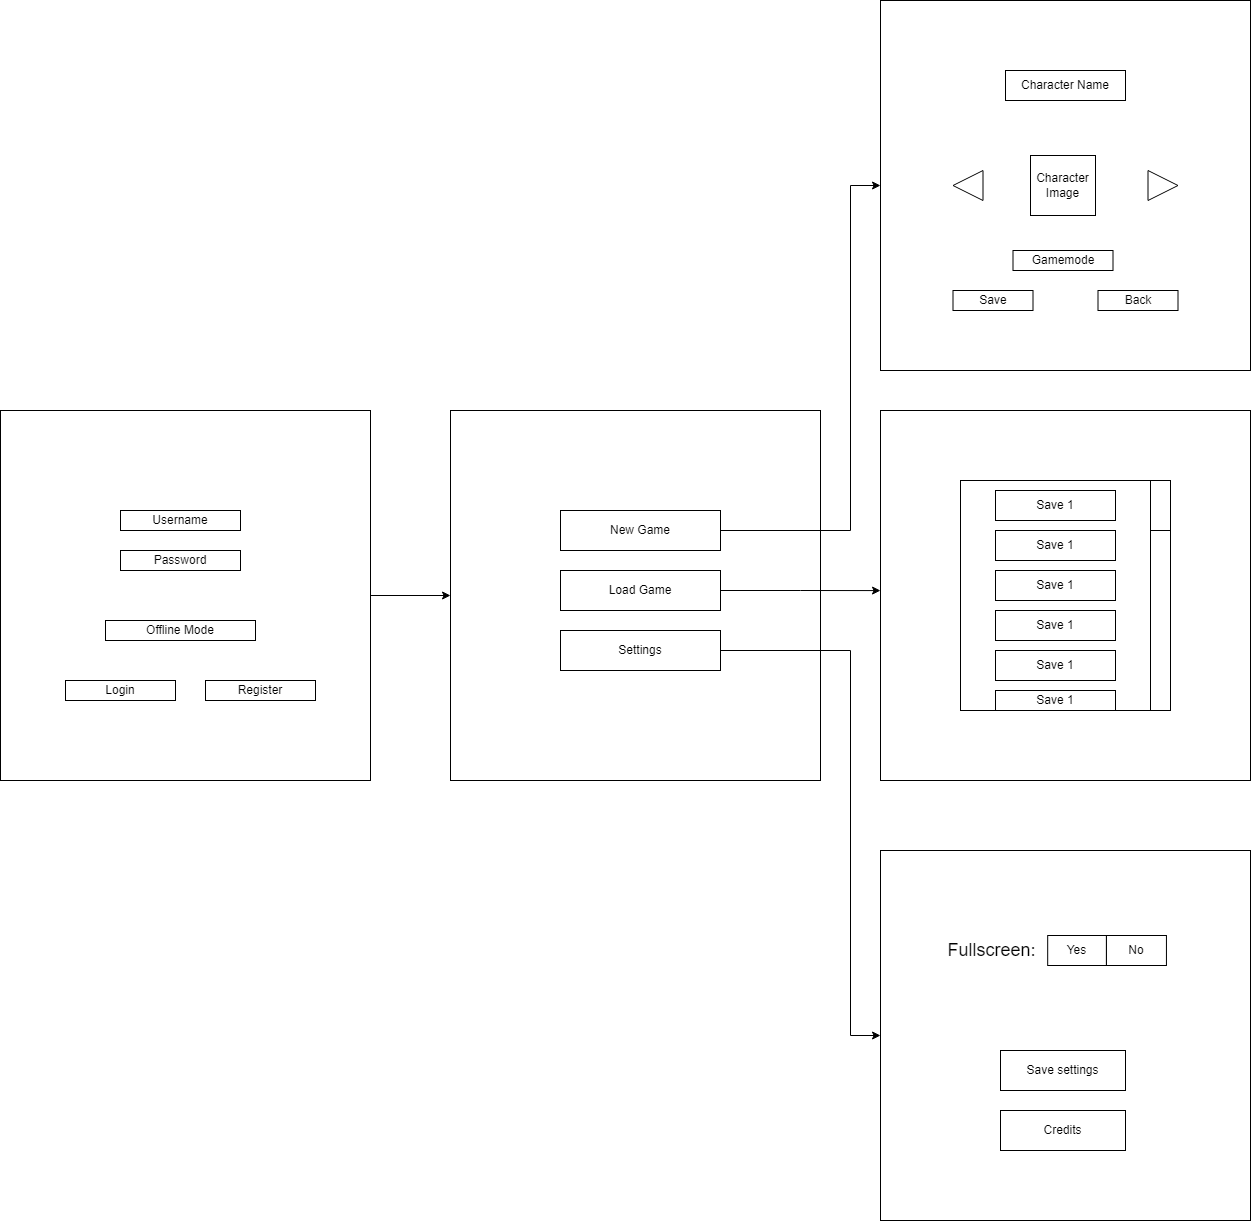
\includegraphics[width=14.0truecm]{images/MS_menu.drawio.png}
    \caption{Menürendszer terve}
    \label{fig:Menürendszer terve}
\end{figure}

\subsection{Felhasználói fiók}
Felhasználói fiók létrehozása azért szükséges a játékomban, mivel szeretnék létrehozni egy ranglista rendszert, ahol a játékosok tudnak egymással versengeni, hogy ki hányszor vitte végig a játékot anélkül, hogy a karaktere egyszer is meghalt volna, miközben a szörnyek minden újrakezdést követően erősödnek. Ehhez a rendszerhez elengedhetetlen, hogy a játékosokat megtudjam különböztetni, illetve, hogy egy adatbázisban eltudjam tárolni a játékosok adatait.

\begin{figure}[H]
    \centering
    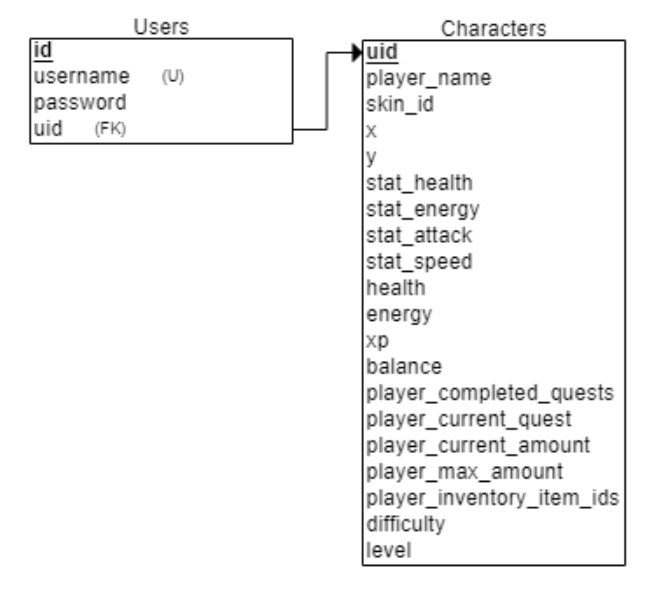
\includegraphics[width=10.0truecm]{images/RelationModell.png}
    \caption{Relációs modell}
    \label{fig:Relációs modell}
\end{figure}

\subsection{Főmenü funkciói}

A bejelentkezést követően a játékosoknak három menüpont fog elérhetővé válni. Az egyik kiemelkedően fontos lehetőség a beállítások menüpont lesz, mivel általában itt találhatók a kulcsfontosságú funkciók módosítására szolgáló lehetőségek. Az én esetemben itt lesz elérhető a teljesképernyős mód beállítása. A beállítások menüpont alatt továbbá megtalálható lesz egy "Credits" opció is, ami tartalmazni fogja a készítő nevét és az elkészítés évét. A másik két menüpontnak pedig a játék indításával kell kapcsolatosnak lennie, mivel a játékosoknak lehetőségük lesz új karakter létrehozására, illetve meglévő mentésük betöltésére.


\subsection{Játékon belüli menürendszer}

A legtöbb játékban kiemelkedő jelentőségű a játékon belüli pillanatálj funkció, valamint egy belső menürendszer. Lényeges, hogy ezek könnyen elérhetőek legyenek, miközben nem zavarják a játékélményt. A játékosoknak lehetőségük lesz a játék közben is hozzáférni egy beállítások menühöz, amelyben a hangerőszintet is be tudják majd állítani. Ezen menü részét kell képeznie egy mentés funkciónak, ami a játék aktuális állapotának mentését teszi lehetővé, továbbá egy folytatás lehetőségnek, és egy kilépés opciónak, amely a játék bezárását szolgálja.


\section{Felhasználói felület és a játékos cselekvési lehetőségei}

A játékokban fontos a jól megtervezett felhasználói felület, amely lehetővé teszi a játékosok számára, hogy a lehető legkönyebben és leggyorsabban elérjék a kívánt funkciókat. Ilyen felület a HUD (Head Up Display)  ez segíti a játékosokat abban, hogy valós idejű információkkal rendelkezzenek a játék világáról, így gyorsabban és hatékonyabban reagálhatnak a különböző helyzetekre.


\subsection{Felhasználói felület}

A felhasználói felület megtervezése során, igyekeztem figyelni, a letisztultságra és a felhasználói élményre. Fontosnak tartottam, hogy a design egyszerű és könnyen átlátható legyen, hogy a felhasználó könnyedén megtalálja azokat a funkciókat és információkat, amelyekre szüksége van.

A HUD (Head Up Display) a játék során folyamatosan látható lesz, így a játékosoknak nem kell külön menübe navigálniuk, hogy megtalálják a szükséges információkat. A HUD a játékos karakterének életpontjait, energia szintjét, a játékos aranyát, a játékos szintjét, a játékos tapasztalati pontjait, a játékos fegyverét, a játékos által használt italokat fogja megjeleníteni.

\begin{figure}[H]
    \centering
    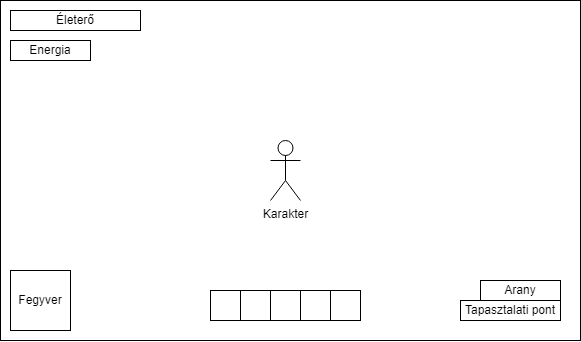
\includegraphics[width=14.0truecm]{images/MS_UI.drawio.png}
    \caption{Felhasználói felület terve}
    \label{fig:Felhasználói felület}
\end{figure}

\subsection{Életpontok és Energia}

A játékos karakterének életpontjai mutatják meg, hogy mennyi sebzést tudnak még elszenvedni mielőtt meghalna a karakterük. Az energia szint pedig a karakter futásához és cselekvéseihez szükséges energiaforrás. A megfelelő kezelése és felhasználása kulcsfontosságú a túléléshez és a harc hatékonyságához.

\subsection{Fegyver Választás}

A játékosnak lehetősége van különböző fegyverek között választani, amelyek különböző képességekkel és támadási stílusokkal rendelkeznek. Ez lehetővé teszi számára, hogy testre szabja a harci stratégiáját és alkalmazkodjon az adott helyzethez.

\subsection{Harcolás Szörnyekkel}

A játék során a játékosnak számos szörnnyel kell megküzdenie. A harcok izgalmasak és változatosak, és a játékosnak ki kell használnia a karaktere készségeit és fegyvereit a sikeres küzdelem érdekében. A szörnyek legyőzése tapasztalati pontokat és esetleges zsákmányt is eredményez.

\subsection{Küldetések Felvétele}

A lineáris történetvezetés lehetőséget kínál arra, hogy a játékosok fokozatosan mélyüljenek el a játék világában, miközben követik a fő cselekményt. A küldetések integrálása a lineáris narratívába lehetővé teszi, hogy a játékosok szorosan kövessék a történet fő vonalát, miközben változatos kihívásokkal találkoznak.

A küldetések kiváló lehetőséget nyújtanak a karakterfejlődésre és a történet gazdagítására. Az XP (tapasztalati pont) és jutalmak rendszere ösztönzi a játékosokat, hogy aktívan részt vegyenek a küldetésekben, és ezáltal fokozatosan erősödjenek a játékban. A lineáris elbeszélésmód segítségével a küldetések sorrendje és nehézségi szintje könnyen szabályozható, így biztosítható a folyamatos kihívás és az érdekesség fenntartása.

\subsection{Italok Vásárlása és Használata}

A játékos aranyat szerezhet a játék során, amit italokra is fordíthat. Az italok különböző hatásokkal rendelkeznek, például életpont visszatöltés vagy energia szint növelés. Az italok stratégiai használata a túlélés és a harcok kulcsa lehet.

\subsection{Statisztikák Növelése tapasztalati pontokból}

A játékos karaktere tapasztalati pontokat szerez a harcok és küldetések során. Az XP felhasználható a karakter statisztikáinak növelésére, például az erő, az ügyesség vagy a mágia terén. Ez lehetővé teszi a karakter fejlődését és a játékmenet testreszabását.

Ezen cselekvési lehetőségek összekapcsolva teremtenek egy gazdag és dinamikus játékélményt az Action RPG játékban, ahol a játékos döntései és cselekedetei hatással vannak a karakter fejlődésére és a játék világára.




\chapter{Megvalósítás}

\section{Grafikák elkészítése}

 Mielőtt nekiláttam a grafikai elemek létrehozásának, inspirációként szolgáltak az interneten elérhető rajzolási stílusok és csempekészletek. Az alapja és mintája a saját rajzaimnak a Ninja Adventure Tileset volt, amelyet Pixel-boy készített.\cite{NAT}

\subsection{Grafikus szerkesztő}

 Fontos kiemelni, hogy egy ``pixelart'' rajz stílusról beszélünk az esetemben, ezért kerestem olyan rajzprogramot, amely minden igényemet kielégíti és könnyen kezelhető tapasztalatlan grafikusok számára is. A kiválaszott program az Aseprite volt, ebben készítettem minden játékban megtalálható grafikát. (Lásd \ref{fig:Aseprite} ábra)

\begin{figure}[H]
    \centering
    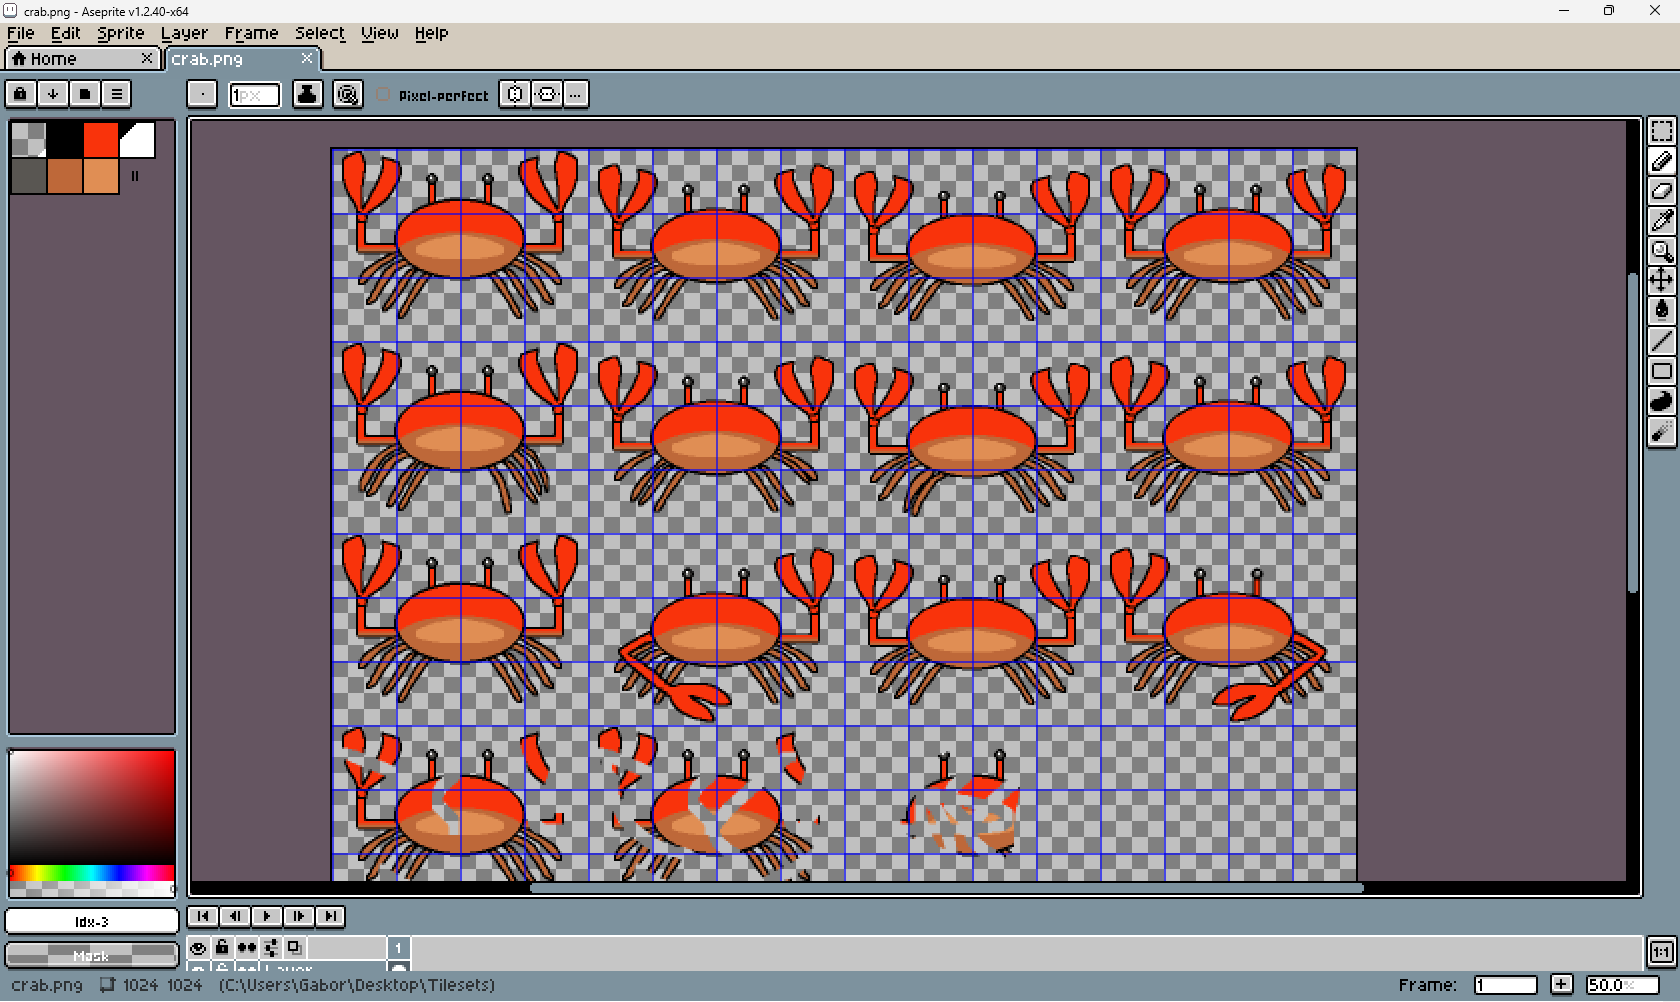
\includegraphics[width=14.0truecm]{images/Aseprite.png}
    \caption{Aseprite - Pixelart rajzoló program
    \cite{Aseprite}}

    \label{fig:Aseprite}
\end{figure}


\subsection{Rajzok elkészítése}

 A rajzok elkészítése két fő részből állt, a pálya tervezéséből és a karakterek, valamint a környezet kialakításából. A pálya tervezéséhez a korábban említett Ninja Adventure Tileset szolgált mintaként, melyből az összes pálya elemét saját kezűleg rajzoltam meg. A karakterek és környezet rajzainak elkészítésénél pedig különböző rajzokat használtam inspirációként, és ezek alapján készítettem el a saját rajzaimat.

\subsubsection{Pálya}
 A pályaelemek létrehozásánál kiemelkedően fontos volt figyelnem arra, hogy a csempék harmonikusan illeszkedjenek egymáshoz, ezáltal kellemes és összefüggő látványt teremtve.

\begin{figure}[H]
    \centering
    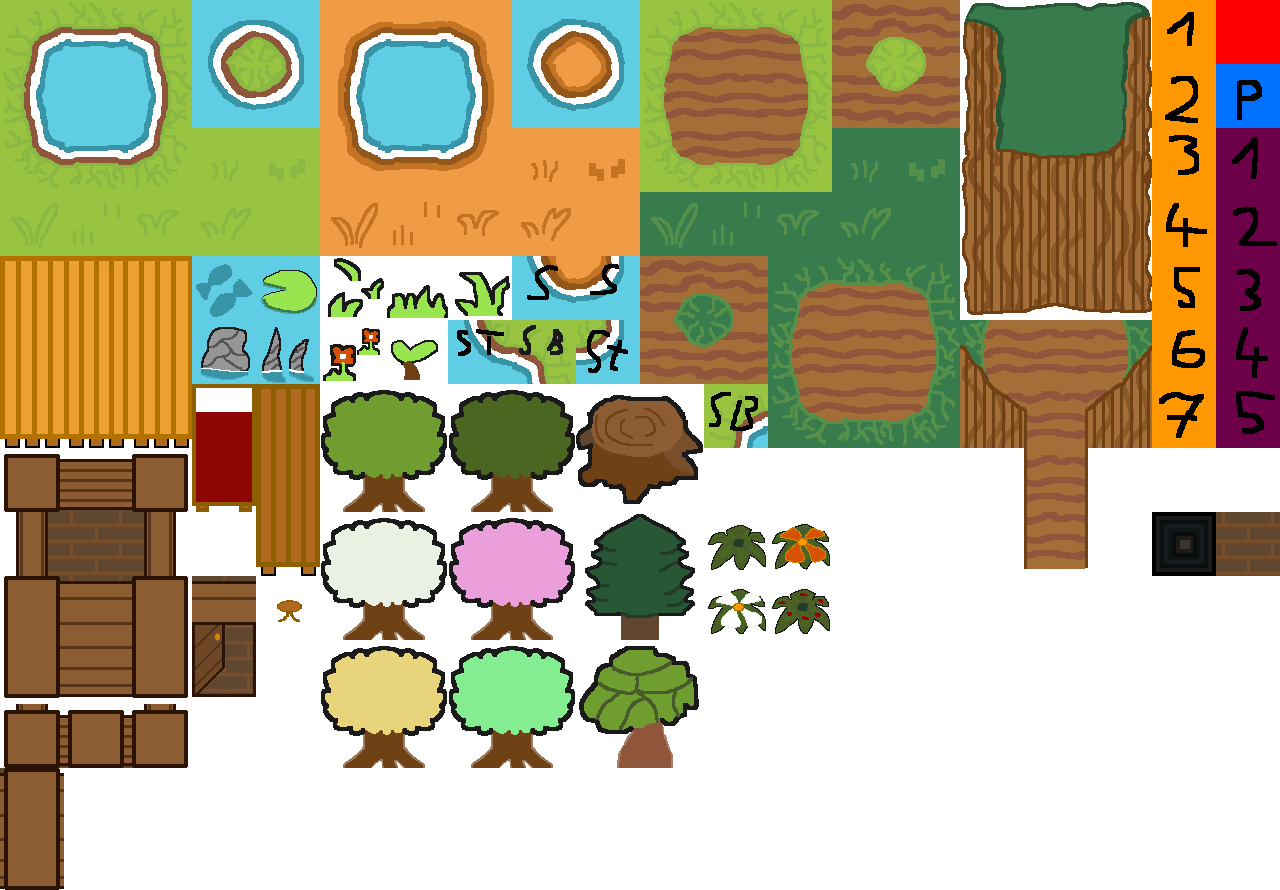
\includegraphics[width=12.0truecm]{images/tileset.png}
    \caption{Csempekészlet}
    \label{fig:Csempekészlet}
\end{figure}

\subsubsection{Entitások}
 Karakterek és szörnyek megtervezése annyiban tért el, hogy ott figyelni kellett az animációra is, mert élethű mozgást szerettem volna utánozni. Egy ilyen mozgás animáció 4-6 képből áll, amelyeket egymás után lejátszva érhető el a kívánt hatás. Illetve, mivel 4 különböző irányba tudnak haladni ezek az entitások, ezért 4 különböző animációt kellett elkészítenem, amelyeket a játék során a karakter irányának megfelelően tudtam lejátszani, ez látható a \ref{fig:Aseprite} ábrán.

\begin{figure}[H]
    \centering
    
\includegraphics[width=12.0truecm]{images/entities.png}
    \caption{Entitások}
    \label{fig:Entitások}
\end{figure}


\section{Pálya megtervezése}

\subsection{Tiled}
\label{subsec:Tiled}
 A pálya megtervezéséhez a Tiled-et \cite{Tiled} választottam, ami egy népszerű térképszerkesztő szoftver, amelyet játékfejlesztők használnak a 2D-s játékok pályáinak tervezésére és szerkesztésére.   A Tiled egy nyílt forráskódú program, így ingyenesen elérhető és széles körben használt az indie játékfejlesztők körében.

Ez a szoftver lehetővé teszi a felhasználók számára, hogy könnyen létrehozzanak és testreszabjanak térképeket, amelyeket különböző játékkeretrendszerekbe integrálhatnak. A Tiled számos funkciót kínál, mint például csempekészletek használata, rétegek kezelése, objektumok lehelyezése rácshálóra, ezzel elkerülve a rétegen belüli átfetéseket. (Lásd \ref{fig:Tiled} ábra) Valamint az exportálás különböző formátumokban, például CSV (Coma-Separated Values) vagy TMX (Tiled Map XML).

Az egyszerű és intuitív felhasználói felülete miatt amit a \ref{fig:Tiled}-es ábrán is lehet látni, a Tiled ideális eszköz a játékfejlesztők számára, akik az apró részletekre is figyelő térképeket szeretnének készíteni játékaikhoz. Az XML alapú TMX formátum kompatibilis a legtöbb játékmotorral, így a Tiled segítségével készült térképek könnyen beilleszthetők a fejlesztési folyamatba.

\begin{figure}[H]
    \centering
    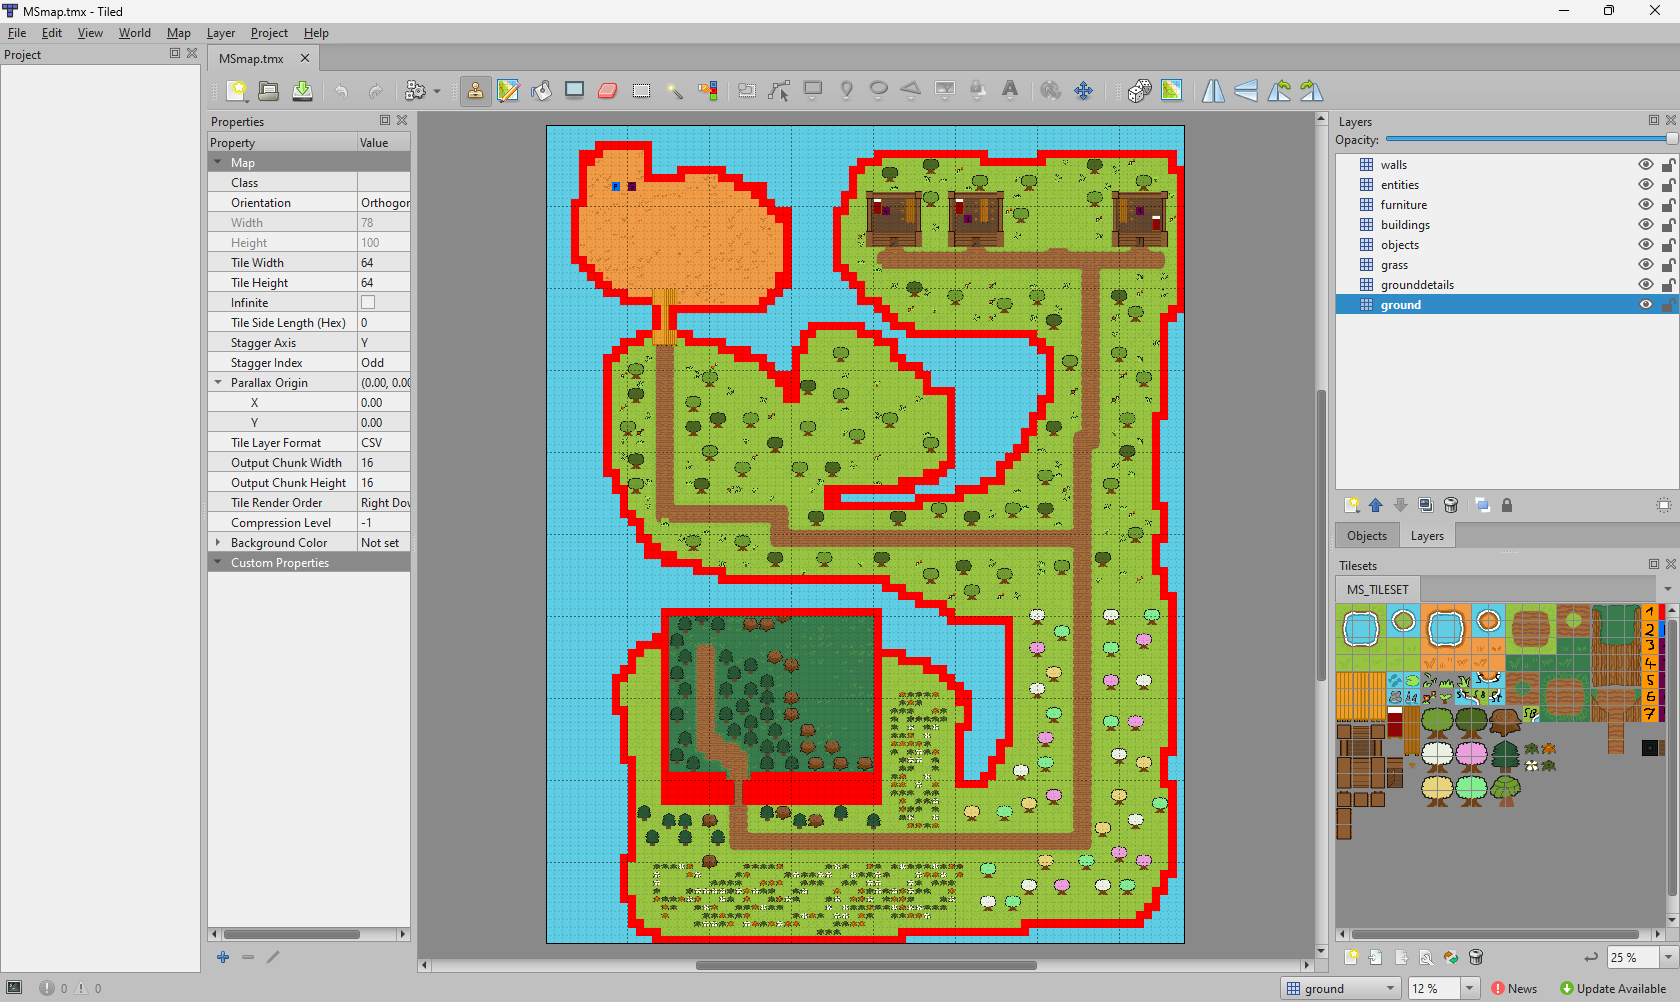
\includegraphics[width=14.0truecm]{images/Tiled.png}
    \caption{Tiled - Pálya szerkesztő
    \cite{Tiled}}
    \label{fig:Tiled}
\end{figure}

\subsection{Tervezés} \label{subsec:Tervezés}

 Kiemelkedően fontos volt a pálya elemeit különböző rétegekre szétválasztani, ezáltal megkönnyítve a fejlesztést és az egyes részek kezelését. A háttér szolgálatában álló csempéket például két rétegre osztottam: az egyikre a talajszintet, a másikra pedig a talajon megtalálható növényzetet helyeztem el. Ezt a két réteget együttesen exportáltam PNG formátumban, amelyet a játékban háttérképként használtam. Fontos megjegyezni, hogy a két háttér réteget nem mentettem külön CSV fájlba. Ennek oka az, hogy ezek a rétegek olyan elemeket tartalmaznak, amelyek statikusak és nincs velük semmiféle interakció a játék során. 

Van még egy fontos réteg amik akadályként szolgálnak a játékos számára (Lásd \ref{fig:Tiled} ábra piroskörvonal), ezeket a rétegeket a játékos nem tudja átlépni, ezáltal a játékmenetet befolyásolják.  

További rétegek lettek létrehozva az objektumok számára, minden típusú objektumot külön rétegen helyeztem el, így könnyen kezelhetőek és nem kell a kódban szűrést alkalmazni a különböző típusú objektumok használatakor.
Réteget hoztam létre a játék során kiüthető objektumoknak, jelenleg a fűcsomók. Nem kiüthető objektumoknak, például házak vagy fák. Berendezési tárgyaknak, mivel azokat talajként szerettem volna kezelni, de nem felülírva a hátteret. Illetve nem utolsó sorban az entitásoknak, hogy milyen pozícióra rajzolja ki őket a játék. (Lásd \ref{fig:Tiled} ábra)

\section{Felhasználói felület és beállítások kezelése}

\subsection{Beállítások}
 A funkció fő célja a beállítások kezelése egy játékban vagy alkalmazásban. Az osztály tartalmazza az alapértelmezett beállításokat, mint például a játékablak méretét, a hangerejét és egyebeket. Az osztály segítségével ezeket a beállításokat be lehet tölteni vagy menteni egy JSON fájlba.

Az ott statikus osztályváltozók az alapértelmezett értékeket tárolják, és a program különböző részeiben felhasználhatók, anélkül, hogy az osztalyt peldanyositani kellene, így könnyen hozzáférhetőek.

További adatokat is tartalmaz, például hangokat, grafikákat, karaktereket, ellenségeket, lövedékeket és fegyvereket. Mindezek az adatok részletezik a játékbeli objektumok tulajdonságait. Azért ezt a megoldást választottam, mert így könnyen kezelhetőek és könnyen módosíthatóak a játékbeli objektumok tulajdonságai. Egyhelyen kezelve egyszerűbb a karbantartás is, ha egy szörny túl erős lenne vagy egy fegyver túl gyenge, akkor csak egy helyen kell módosítani az adatokat, és az összes példányban azonnal érvényesülnek a változtatások.

Az osztály emellett definiálja a felhasználói felület színeit és stílusait, amelyek a játék megjelenítéséhez használok. Ez azért fontos, hogy egységes megjelenést biztosítson a felhasználói felületben, és ahogy az előbb is említettem, egy színkód megváltoztatásával mindenhol azonnal érvényesül a változtatás.


\subsection{Felhasználói fiók}
 Ez a rendszer kezeli a regisztrációhoz és a bejelentkezéshez kapcsolódó folyamatokat. Ilyen folyamat többek között a felhasználói felület megjelenítése, de a tartalomellenőrzés és hibakezelés is. Tartalomellenőrzés alatt a felhasználónév és jelszó validálás értendő, hogy megfelelő formátumban vannak-e megadva. Hibakezelés alatt pedig a felhasználó értesítése, ha valamilyen hiba történik a regisztráció vagy bejelentkezés során. regisztráció esetén, ha sikeres validálás történik, akkor md5 hash algoritmus segítségével titkosítva tárolja a jelszót az adatbázisban. Bejelentkezéskor ezt a titkosított jelszót hasonlítja össze a felhasználó által megadott jelszó titkosított formájával, ha megegyezik, akkor engedi a bejelentkezést.

\subsection{Főmenü}

 A játéknak elengedhetetlen része a főmenü, ami a bejelentkezés után válik elérhetővé a felhasználók számára. Biztosítok a játékosoknak offline, azaz internet nélküli játszási lehetőséget, ilyenkor regisztráció és bejelentkezés nélkül használni lehet a játékot.
A főmenüben legfelül a játék címe ``Marooned Sailor'' jelenik meg, alatta három menüpont található meg, az új játék létrehozása, meglévő mentés betöltése, illetve a beállítások. Kijelentkezési lehetőséget nem valósítottam meg, ahogy kilépés gombot sem helyeztem el, ezzel szeretném ösztönözni azokat akik kipróbálják, hogy ne zárják be első látásra a játékot. Bezárni az asztali alkalmazást a pillanat állj menüben lehet majd a játék során az exit menüpontra kattintva. (Lásd \ref{fig:Főmenü} ábra) 

\begin{figure}[hbt]
    \centering
    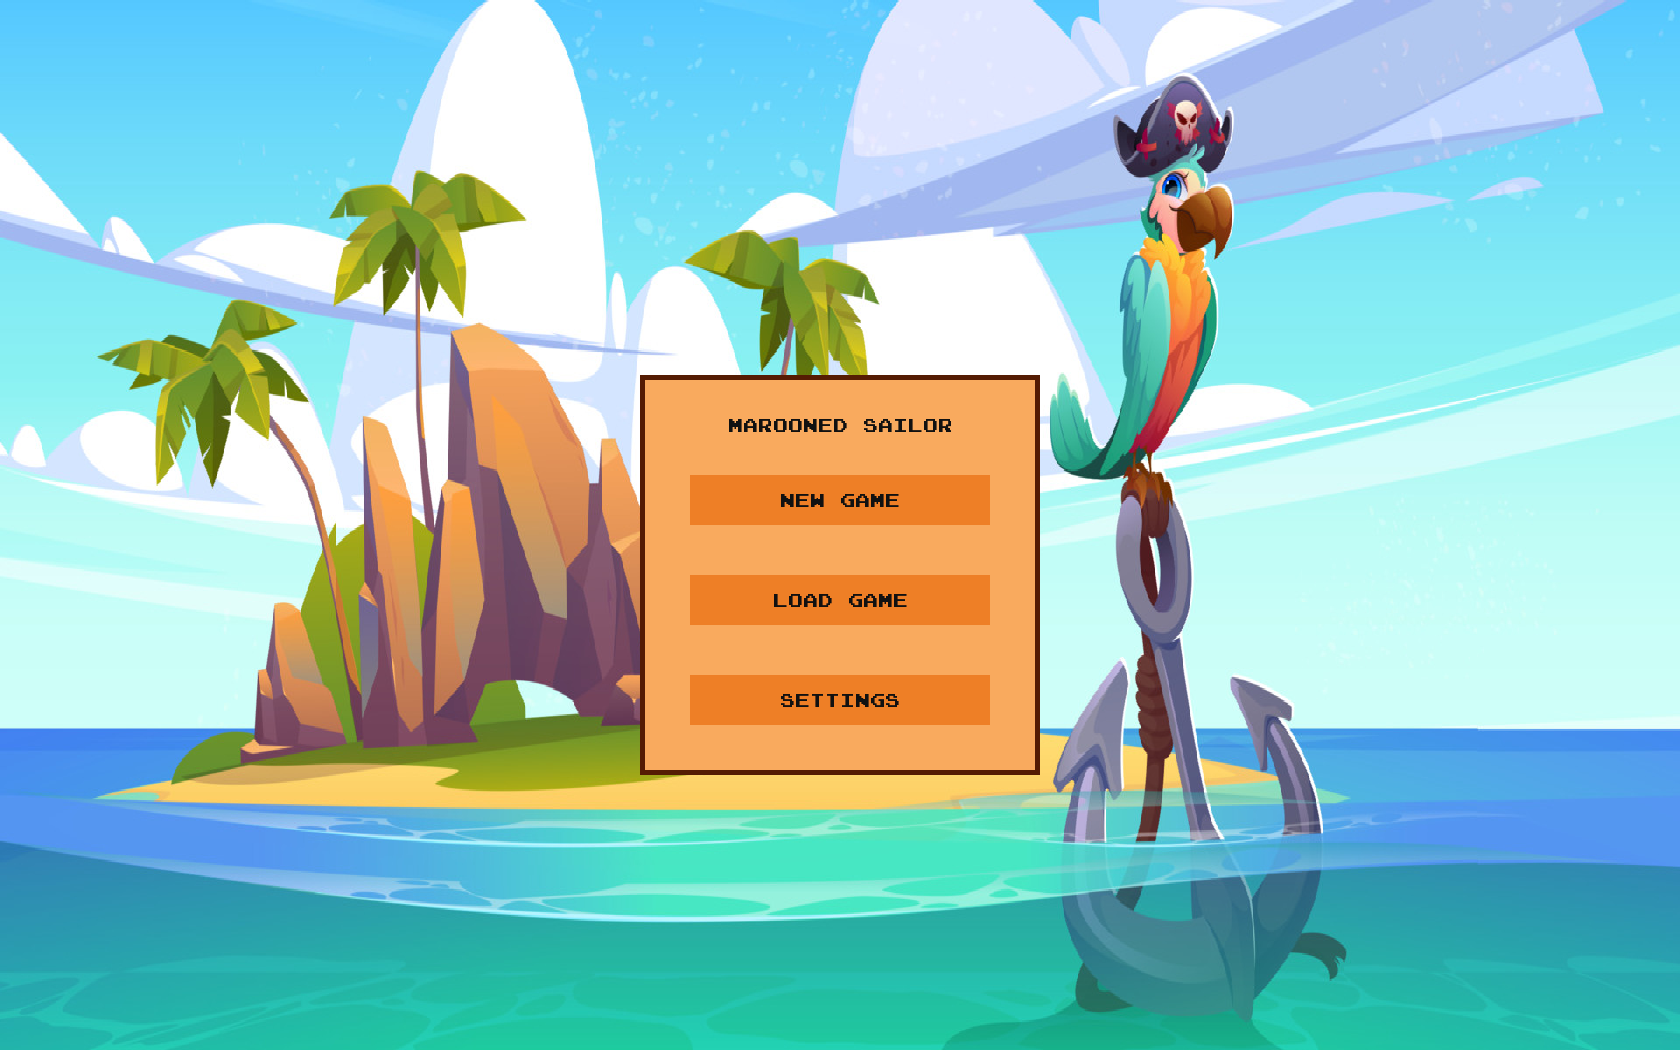
\includegraphics[width=14.0truecm]{images/mainmenu.png}
    \caption{Főmenü}
    \label{fig:Főmenü}
\end{figure}


\subsection{Új játék létrehozása}
 Az új játék menüpont kiválasztása után (lásd \ref{fig:Új játék létrehozása}) a játékosnak meg kell adni a karakterének a nevét, illetve választhat különböző karakter kinézetek közül. Ha be van jelentkezve a játékos, akkor van lehetősége nehézségi szintet is választani.
A nehézségi szint annyiban különbözik, hogy a ``normal'' módban, ha elfogynak a játékos életpontjai, akkor a játék folytatódik tovább, újraéled egy bizonyos helyen. Viszont, ha a ``challange'' (kihívás) módot választja, akkor három funkcióval bővül a játékmenet. Az első ilyen funkció, hogy ha elfogy a játékos életereje, akkor véglegesen meghal a karakter, és nem lesz lehetősége tovább folytatni azzal a bizonyos karakterrel a játékot. A második plusz funkció, hogy az összes küldetés teljesítése esetén a játék újrakezdődik, amely azt eredményezi, hogy a szörnyek erősödnek, és nagyobb kihívás lesz újra végigvinni az összes küldetést. Illetve tartalmaz egy ranglista menüpontot, amely jelzi a legügyesebb játékosok hányszor tudták a ``challange'' mód használatával végigvinni az összes küldetést. (Lásd \ref{fig:Új játék létrehozása} ábra)

\begin{figure}[H]
    \centering
    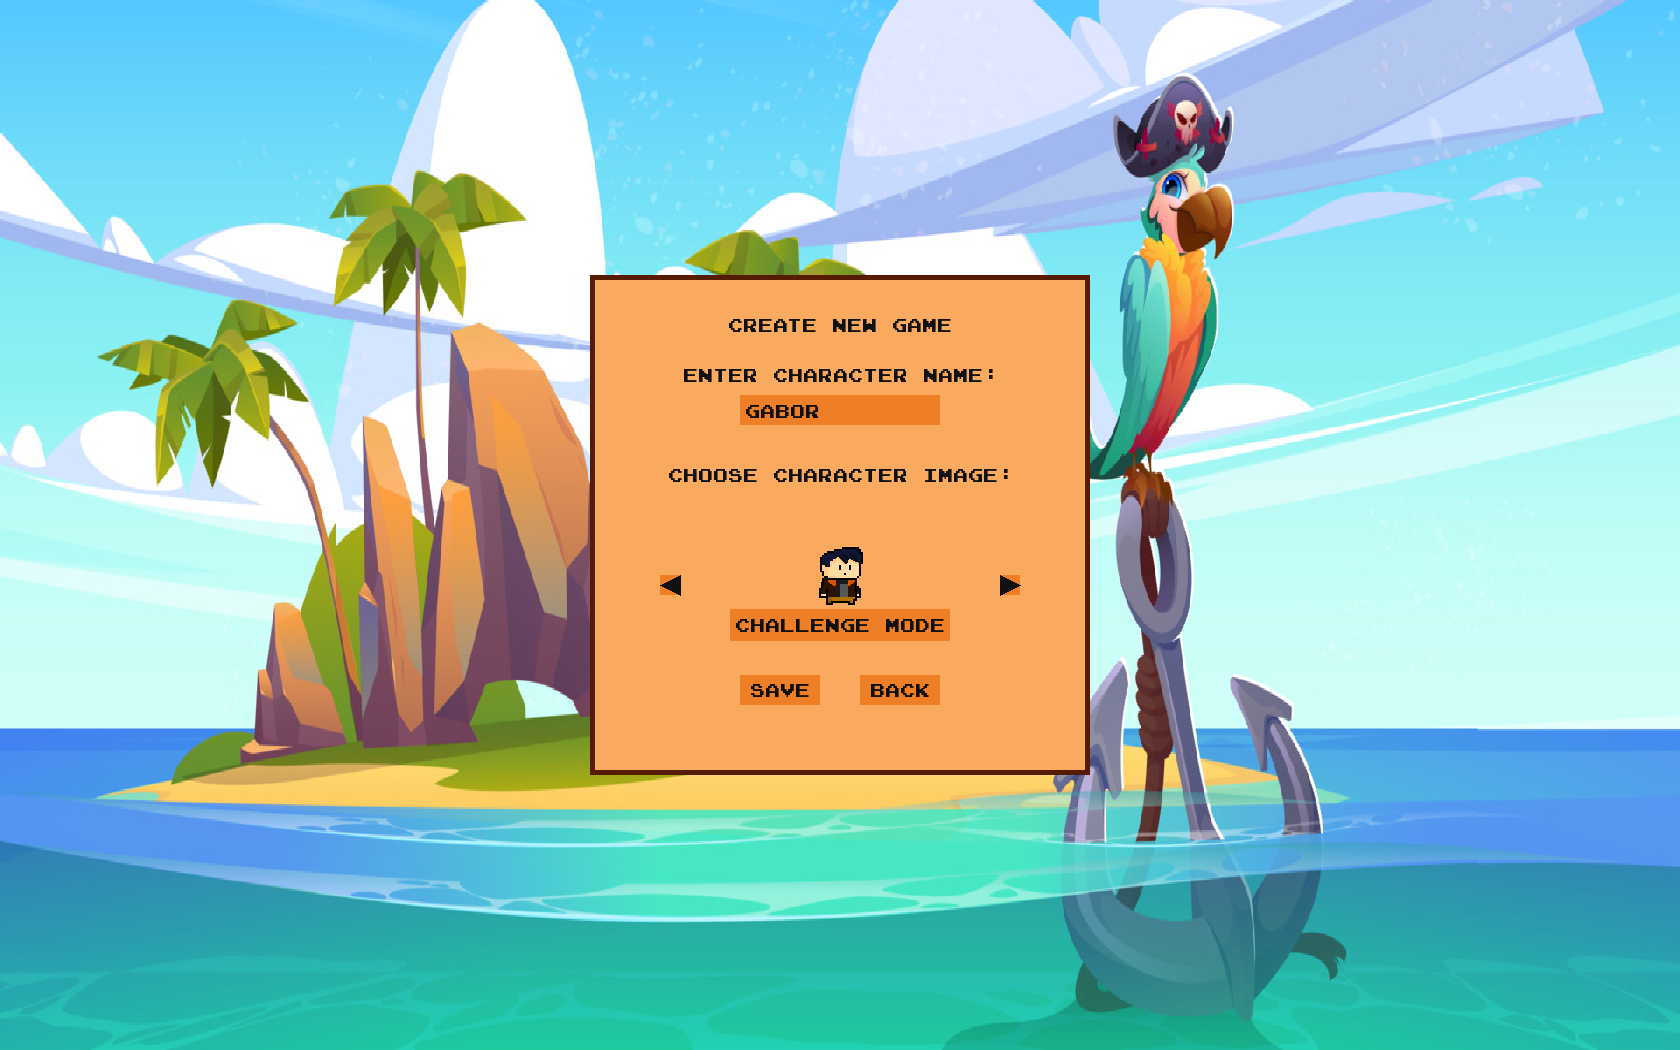
\includegraphics[width=14.0truecm]{images/newgame.png}
    \caption{Új játék létrehozása}
    \label{fig:Új játék létrehozása}
\end{figure}

\subsection{Játékmenet közbeni menü}
 Az Esc gomb megnyomásával elérünk egy pillanat állj funkciót, amely egyben egy menüt is megjelenít, ahol a játékosnak lehetősége van a játékállapot mentésére. Illetve folytatni a játékot vagy kilépni az asztalra. (Lásd \ref{fig:Játékmenet közbeni menü})

A pillanat állj funkciót úgy valósítottam meg, hogy az összes játékbeli sprite group, azaz felületi csoport (később bővebben lesz szó ezekről \ref{subsec:Pálya kezelése}) kirajzolására szolgáló függvényt állítom le egy boolean típusú változóval, ezáltal minden játékon belüli elem megáll a legutolsó ismert állapotában, majd a menü bezárása után, amelyet a resume (folytatás) gomb megnyomásával tehet meg a játékos, onnan folytatódnak az események, ahol abbamaradtak.


\begin{figure}[H]
    \centering
    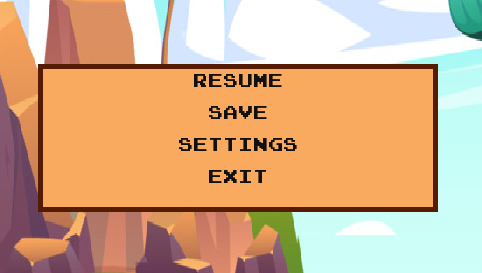
\includegraphics[width=12.0truecm]{images/ingamemenu.png}
    \caption{Játékmenet közbeni menü}
    \label{fig:Játékmenet közbeni menü}
\end{figure}

\subsection{Mentések betöltése}
 A játékosnak lehetősége van a korábban elmentett játékállás betöltésére is, amennyiben van ilyen. A betöltés után a játék onnan folytatódik, ahol abbahagyta. Egy lista elrendezésben látja a felhasználó a korábbi mentéseit. Előre rendezi az offline mentéseket a listában, és csak utánuk tölti be az online mentéseket. Egy kattintás után már be is tölti az adott játék állást. Külön nem jelzi, hogy az adott mentés melyik kategóriába tartozik, egyszerűen nem jelennek meg a listában az online mentések, ha nincs bejelentkezve a felhasználó.

\section{Játékmenet kezelése}

\subsection{Main metódus}
 Ez az osztály felelős a játék főciklusának végrehajtásáért, ami az egész játék működésének alapját képezi. Amikor a játék elindul, az alkalmazás példányosítja ezt az osztályt.

A \ref{py:főciklus} programkód részletesen bemutatja, hogyan kell megvalósítani ezt a főciklust, amely a játék működéséért felelős. Ebben a kódban kezeljük a játék fő eseményeit, és gondoskodunk arról, hogy minden szükséges műveletet végrehajtsunk a játék folyamán.

Amikor elindul a játék, a bejelentkezési képernyőt találjuk magunkat. A menuenums enum típusban tárolt értékek segítségével dönti el a program, hogy mely állapotot kell megjeleníteni. Itt gondolok, a bejelentkezési képernyőre, főmenüre és annak almenüire, illetve a játékra magára. 

A főciklusban történik, a képrissítés mértékének beállítása a self.clock.tick(Settings.FPS) sorral, az ablak háttérszínének beállítására a self.screen.fill(Settings.WATER\_COLOR) sorral, a játékmenet futtatására a self.game\_handler.run() sorral, és a képernyő frissítésére a pygame.display.update() sorral.

Tehát létfontosságú szerepet játszik abban, hogy a játék működése zökkenőmentes legyen, és a kódban látható példa segítségével könnyen megérthető, hogyan történik mindez.


\begin{python}[caption={Játék főciklusa},label=py:főciklus]
    def run(self):
        while True:
            [...]
            elif self.state == menuenums.GAME:
                if self.game_handler is None:
                    Sounds.play_loop('main')
                    self.game_handler = GameHandler(
                        self.user, self.save_parameters)
                for event in pygame.event.get():
                    if event.type == pygame.QUIT:
                        pygame.quit()
                        sys.exit()
                self.screen.fill(Settings.WATER_COLOR)
                self.game_handler.run()
                pygame.display.update()
                self.clock.tick(Settings.FPS)
\end{python}

\subsection{Játékon belüli felületek} \label{subsec:A játék fő osztálya}
 A GameHandler osztály, nagyon fontos szerepet tölt be a játék futása során, több alapvető funkciót kezel. Ez az osztály kezeli a mentéseket erről a későbbiekben \ref{subsec:Játékállapot mentése} szakaszban tárgyalunk majd. 
Kezeli a megjelenített felületeket, értem ezalatt a játékmeneten belüli menüt, ez valósítja meg a pillanat állj funkciót is. Mivel megállítja a LevelHandler (erről a \ref{subsec:Pálya kezelése} szakaszban lesz szó) álltal frissített felületeket. Itt kezelt felület a ranglista funkció, amely a játékmenet megállítása nélkül is látható. Az utolsó általa kezelt felület a karakter fejlesztési panel is, amely a játékos karakterének fejlesztésére szolgál.

\subsection{Játékállapot mentése} \label{subsec:Játékállapot mentése}
 A játékállapot elmentését Save gomb megnyomásával lehet elérni. A mentés a játékállapot minden fontosabb elemét eltárolja egy JSON típusú fájlban, ha offline módban játszik a játékos, vagy FastAPI-on \cite{fastapi} keresztül kommunikálva egy MySQL \cite{mysql} adatbázisban, ha online módot választott a felhasználó. 
Minden karakterhez egy mentési lehetőség tartozik, tehát nem lehet egy karakterhez több játékállapotbeli mentést készíteni. Mindig az utolsó mentés kerül felülírásra, ha a játékos új mentést készít. Ebből következik, hogy a játékosnak mentéskor nincs lehetősége rálátni a korábbi mentéseire, csak a betöltési menüben, ahol a játékos kiválaszthatja a korábbi mentéseit.

\subsection{Pálya kezelése} \label{subsec:Pálya kezelése}
 Levelhandler a másik nagyon lényeges osztály, ez a GameHandler-ben kerül példányosításra. Feladata a világok, a kamera, entitások létrehozása és kezelése ellentétben a GameHandler osztállyal (Lásd \ref{subsec:A játék fő osztálya}) amely feladata a játékon belül elérhető funkciók kezelése, értem ezalatt a menük megjelenítését, mentést vagy a pálya futtatását. 
Ezeket a különböző felületeket Sprite Group-okba szervezve kezeli, így könnyen tudja őket elérni és frissíteni. Ezeket a csoportokat a Tiled-ben létrehozott rétegek alapján határozza meg, milyen felület milyen jellemzőkkel fog rendelkezni.
Legfontosabb ezek a sprite csoportok közül talán a Visible Sprite csoport, amely a játékos által látható felületeket tartalmazza. A kamera ezeket rendereli ki úgy, hogy ezeket a csempéket y tengely szerint rendezi és úgy jeleníti meg, hiszen, ha az alapértelmezett x tengelyen haladna végig a kirajzolási funkció, akkor nem lehetne elérni hamis 3D hatást. Jelenleg, ha a karakter egy fa ``felett'' tartózkodik azt félig rá rajzolja ki ezáltal elérve mintha mögötte bújkálna a karakter, de ez minden elérhető felületre igaz. Maradva az előző példánál, ez x tegnely szerinti rendezésben esetében úgy nézne ki, hogy a karakter a fa baloldalánál állva a fa mögött helyezkedne el, azaz a karaktert kitakarná, ameddig a jobb oldalán a karakter lenne az előtérben. 
Megtalálható még obstacle (akadály), attack (támadó), és attackable (támadható) felület csoportok is, amelyek a játékmenet során fontos szerepet játszanak, különböző mechanikák végrehajtásánál. Az obstacle csoportba \ref{fig:Tiled} ábrán piros körvonalú rétegen szereplő csempék kapták, amelyek szerepe, hogy az ütközésvizsgálat ebbe a csoportba tartozó csempéket veszi figyelembe. Az attack csoportba a játékos által irányított karakter támadó felületei kerültek azaz a fegyverek, hiszen ezeket nagyon rövid ideig kell megjeleníteni ezután törölni azokat. Az attackable csoport szorosan kapcsolódik az utóbb említett csoporthoz. Ide tartozik az összes olyan felület, amelyekkel a fegyverek interakcióba kerülhetnek. Ebbe a csoportba tartoznak például a szörnyek, de a fűcsomók is amelyeket a játékos ki tud ütni a fegyverével. 

\subsection{Világ és barlangok} \label{subsec:Világ és barlangok}

 A játékos amikor létrehoz egy új karaktert, vagy beölt egyet akkor egy világban fogja találni magát. Ez a világ a fő pályarész, itt helyezkedik el minden kulcsontosságú helyszín és karakterek. Illetve a játék során ellehet látogatni egy barlangba ami egy nagyságrendileg kisebb terület, amelyből több is létezhet egy világban.
 A world és a dungeon osztály közös szülő osztályból származnak le, ez azért fontos, hogy a különböző világokat könnyen tudjam kezelni
 és különböző tulajdonságokat adni nekik. Ebben az osztályban a minden világra vonatkozó lehetőségeket kezelem, ilyen például
  az effekteket lejátszó AnimationPlayer osztályom származtatása, mert azt elég egyszer definiálni és meghívni ott, ahol szükséges, ahelyett,
   hogy minden világnak lenne egy külön példánya. Továbbá ilyen opció a térképmegnyitás, és az azzal kapcsolatos összes funkció,
    például, hogy hol található a következő küldést adó nem játékos karakter. A játék története jelenleg teljesen lineáris,
     tehát egy adott sorrendben történhet csak a küldetések teljesítése. Ez az osztály kezeli szörnyek legyőzése által elejtett, hátrahagyott tárgyakat, ilyen tárgyak a tapasztalati pont és az aranypénz.
       Ezeket a tárgyakat a játékos össze tudja gyűjteni, és a későbbiekben fel tudja használni.  

\subsubsection{Pálya generáláshoz szükséges adatok} \label {subsec:Pálya generáláshoz szükséges adatok}

 Említettem a korábbi fejezetben, a pálya megtervezését a \textbf{Tiled}-el végeztem. (Lásd \ref{subsec:Tiled}) 
Első megközelítésemben CSV (vesszővel elválaszott értékek) fájl formátumba mentettem ki a tervezőben létrehozott rétegeket. Egy ilyen dokumentum úgy néz ki, hogy ahova nem helyeztem le a tervezőben objektumot, ott '-1' érték szerepel, ellentétben ahol van érték, ott a Tiled-ben betöltött és feldarabolt csempekészlet azonosító számai kerültek a dokumentumba. Ezt úgy kell elképzelni, mint egy nagy mátrixot. Az utolsó pillanatokig ezt a megközelítést alkalmaztam, mert ha már kész volt és működött, miért változtattam volna rajta. Végül mégis visszatértem erre a kérdéskörre és készítettem az alább olvasható kis egyszerű átalakító szkriptet. (Lásd \ref{py:csvtodict} programkód) Ennek funkciója, a sok felesleges '-1' értéket kiszűrni, hogy a program futása közben ne kelljen a betöltésnél rengeteg felesleges összehasonlítást végezni. Ezt úgy oldottam meg, hogy készítettem python dictionary-t a csempe azonosító számából, illetve annak a .CSV mátrixban elhelyezkedő koordinátáiról. (Lásd \ref{py:átalakított struktúra} programkód)


\begin{python}[caption={CSV formátum dictionary formátumra konvertálása},label=py:csvtodict]
    import csv
    import json
    
    csv_file = "new_map\MSmap._dungeonentrance.csv"
    map_data = []
    
    with open(csv_file, newline='') as csvfile:
        csv_reader = csv.reader(csvfile)
    
        for i, row in enumerate(csv_reader):
            for j, value in enumerate(row):
    
                value = int(value)
                if value != -1:
                    map_data.append({"i": i, "j": j, "value": value})
    
    python_file = "world_dungeonentrance"
    
    with open(python_file, 'w') as pyfile:
        pyfile.write("map_data = ")
        json.dump(map_data, pyfile, indent=4)
    
    print(f"Dictionary saved to {python_file}")
    
\end{python}


Készítettem egy kis függvényt, a pálya létrehozásának idejének lemérésére. Ez azért volt fontos, hogy megtudjam határozni, hogy a szótár használata jobb megoldás-e, mint a CSV fájl. A két megoldás esetében a következő eredményeket kaptam:

\begin{itemize}
    
    \item Python dictionary esetében:
    \begin{verbatim}
        Futási idő: 108.64 ms
    \end{verbatim}
    \item Comma-Separated Values (CSV) esetében:
    \begin{verbatim}
        Futási idő: 879.92 ms
    \end{verbatim}
\end{itemize}
    
 Tehát elmondható, hogy ez a változtatás jelentősen felgyorsította a pálya létrehozását, ezáltal a játék betöltési ideje is csökkent.



\begin{python}[caption={Minta az átalakított struktúrára
    }, label=py:átalakított struktúra]
    {
        "i": 3,
        "j": 41,
        "value": 125
    },
\end{python}

\subsubsection{Pálya generálás}

 A korábban (lásd \ref{subsec:Tervezés}) megtervezett és exportált majd feldolgozott (Lásd \ref{subsec:Pálya generáláshoz szükséges adatok}) pályaadatok megjelenítését több lépésben valósítottam meg. Először is a képeket be kell tudnom olvasni, ezt az os \cite{Python-os} könyvtár walk függvényének segítségével oldottam meg.
 Miután sikerült bejárni a mappát, előállította az egyes képekhez vezető útvonalat, ezután a pygame.image.load() függvényével betölti a képeket. A képeket entitás esetében képkockánként, míg a pálya esetében mozaik-kockák formájában tároltam.
  Ezt követően a képeket egy listába helyeztem, amelyet később fel tudok használni a kirajzoláshoz.
   Másik ilyen fontos lépés a pálya rétegek beolvasása, amelyet a korábban említett dictionary segítségével valósítottam meg.
    Ezután egy ciklusban végig iterálva a dictionary-n, a képek listájából kiválasztotta a megfelelő képet, és a megfelelő koordinátákat,
     amelyeket segítségével példányosítom a Tile osztályt, később ennek segítségével végzi el a kirajzolást.
      Mivel a szótárak között szerepel az entitásokra vonatkozó réteg is, ezért azokat is az előbb említett iterációban kezeltem,
       és példányosítottam a hozzájuk tartozó osztályokat, azonosító alapján szűrve.

\subsection{Entitások} \label{subsec:Entitások}
 Ez az osztály egy szülő osztály amit az Enemy, NPC és Player osztályok használnak. A szülő osztály azt jelenti, hogy ebből származnak le más osztályok és felhasználják minden tulajdonságát, illetve metódusait is.  

Három fontos metódussal rendelkezik, az egyik a mozgás kezelése. A mozgást a move függvény segítségével hajtja végre, amelynek a lényege, hogy az entitás rendelkezik egy irány változóval, ami tárolja, hogy merre néz (ez lehet fel, le, jobbra, balra), és ezeknek az irányoknak a vektorának normalizálásával és a paraméterként megkapott sebesség értékkel meghatározza a következő pozícióját az entitásnak. A normalizás azért fontos, hogy átlós mozgás esetén ne mozogjon az adott karakter sokkal gyorsabban. A vektor egységesítéséhez, normalizálásához a vektor minden egyes komponensét el kell osztani annak hosszával, ezzel elérve, hogy a vektor iránya ne változzon, csak a hossza legyen 1. A pozíció módosítás az egyed hitbox-ára vonatkozik, azaz arra a dobozra, amely az entitást körülveszi. Azért a hitbox-ot kell mozgatni, mert a szörnyek és karakterek képei a hitboxra vannak igazítva. Ez azért fontos, mert így megelőzhető az olyan hibák előfordulása, amit a hitbox és a kép közötti eltérés okozhatna. Ilyen szinkrinizációs hiba, például lövöldözős játékok esetében szokott látványosan előfordulni, hogy egy bizonyos testrész hitbox-a nem ott helyezkedik el ahol a grafika, és a játékosok miközben látják, hogy eltalálják az ellenfelet, mégsem történik sebzés.

A másik egy szinusz függvény alapján ad vissza 0-255 értéket, ez arra szolgál, hogy az elszenvedett sebzés után villogó effekt játszódjon le az adott entitáson, ezzel jelezve meddig sebezhetetlen. A harmadik metódus az ütközés érzékelésre, kezelésére szolgál.

Az ütközés érzékelés lényegében úgy működik, hogy nézzük az entitás mozgási irányát, hogy függőlegesen, vagy vízszintesen közlekedik, és az adott iránytól függően vizsgáljuk, hogy az entitás fizikai kiterjedése (későbbiekben hitbox), esetemben egy grafika nagyságú téglalap ütközik-e valamelyik korábban említett obstacle, akadály csoport csempével. Ha igen, akkor az entitás irány szerinti hitbox határát az akadály ellenkező irányű hitbox határához igazítjuk, így megakadályozva az áthaladást, de nem letiltva a többi irányba való mozgást. (Lásd \ref{fig:Ütközés kezelése} ábra, és \ref{py:Ütközés kezelés} programkód)




\begin{python}[caption={Ütközés kezelése},label=py:Ütközés kezelés]
def collision(self, direction):
    #horizontalis mozgas
    if direction == 'horizontal':
        for sprite in self.obstacle_sprites:
            if sprite.hitbox.colliderect(self.hitbox):
                if self.direction.x > 0:
                # jobbra mozgas
                    self.hitbox.right = sprite.hitbox.left
                if self.direction.x < 0:
                # balra mozgas
                    self.hitbox.left = sprite.hitbox.right                   
    #vertikalis mozgas
    if direction == 'vertical':
        for sprite in self.obstacle_sprites:
            if sprite.hitbox.colliderect(self.hitbox):
                    if self.direction.y > 0:
                        # lefele mozgas
                        self.hitbox.bottom = sprite.hitbox.top
                        if self.direction.y < 0:
                        # felfele mozgas
                        self.hitbox.top = sprite.hitbox.bottom
                    \end{python} 


                    \begin{figure}[H]
                        \centering
                        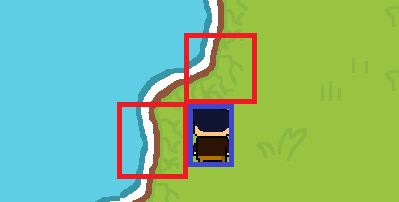
\includegraphics[width=15.0truecm]{images/collision.png}
                        \caption{Ütközés kezelése}
                        \label{fig:Ütközés kezelése}
                    \end{figure}
                    
                    
\subsection{Játékos karaktere}
 Ez az osztály a játékos karakterét valósítja meg, amely a játék során irányítható. A játékos karaktere egy entitás, így örökli az entitás osztály összes tulajdonságát és metódusát.

Az osztály inicializálása során számos fontos adatot tárol, például a játékos nevét, karakterének azonosítóját és kezdeti pozícióját. Ezek az adatok meghatározzák a karakter kezdeti állapotát a játékban.

A karakter mozgását és irányítását az osztály input metódusa kezeli. Ennek segítségével az osztály figyeli, hogy milyen billentyűk vannak lenyomva, és ennek megfelelően mozgatja a karaktert a játékban. A játékos karakter képes balra, jobbra, felfelé és lefelé mozogni a megfelelő billentyűk lenyomásával.

A karakter sebessége és energiaszintje dinamikusan változik a játék során. Például a karakter gyorsabban mozoghat, ha lenyomja a ``SHIFT'' billentyűt, és az energia szintje csökken mindeközben. Az energia idővel regenerálódik, ami lehetővé teszi, hogy tovább használhassa a gyors futás funkciót.

A játékos karakter képes támadni is, és az attack metódus meghívásával hozza létre a támadást. A támadásokat az osztály figyeli, és számítja ki a támadások között eltelt időt, hogy ne lehessen túl gyorsan ütni a fegyverekkel.

A karakter fegyvere is dinamikusan változik, és a játékos lehetőséget kap a fegyver cseréjére a játék során.

A karakternek vannak életpontjai és energia szintje, amelyek meghatározzák a túlélését a játékban. Amennyiben az életpontja nullára csökken, a karakter meghal, de van lehetőség a visszatérésre vagy újrakezdésre a játékban, attól függően, hogy milyen a játék nehézségi szintje.

A karakter számos egyéb tulajdonsággal és képességgel rendelkezik, például tapasztalati pontokkal, megszerzett arany mennyiségével és teljesített küldetésekkel. Ezek a tényezők befolyásolják a játékmenetet és a karakter fejlődését.

Az osztály továbbá lehetővé teszi a karakternek, hogy tárgyakat használjon és rendelkezzen egy táskával. A játékos képes tárgyakat váltani és használni a játék során, ami további taktikai elemet ad a játékhoz.

Összességében ez az osztály kulcsfontosságú a játékos karakter kezelésében és irányításában, lehetővé téve a játékosnak, hogy részt vegyen a játék világában és kihívásokkal nézzen szembe a karaktere fejlesztése során.

\subsection{Fegyverek}

 A különböző fegyverek (Lásd \ref{fig:A játékban megtalálható fegyverek} ábra) használata szintén egy elengedhetetlen része a játéknak. A fegyvereket a játékos karaktere használja a szörnyek elleni harc során. Közlehraci fegyvereket valósítottam meg, a kard, a lándzsa, a kétkezes kard és a kétkezes lándzsa. Ezek a fegyverek különböző támadási távolsággal és sebzéssel rendelkeznek, előkészítettem a támadási sebesség megvalósítását is, de az végül nem került be a játékba, mert szerintem rontotta volna a játékélményt.

Ezen harcolásra szolgáló eszközök kirajzolása a támadás gomb lenyomása után történik a Weapon osztály példányosításával. Ez az osztály a játékos karaktere által kezében tartott fegyvert rajzolja ki a képernyőre. Mivel fontosnak tartottam, hogy mozgás közben is lehessen támadni, illetve legyen egy csapás/suhintás animáció, ezért egy frissítés funkciót vezettem be, amely mindig a játékos karakterének legutóbbi helyzetét, és irányát vizsgálja, majd ezekre az adatokra alapozva frissíti a már létrehozott képet. A csapás animációt mind a négy irányban külön-külön kellett megtervezni, mert a fegyverek nem egyformán néznek ki minden irányból. Szinusz függvény segítségével valósítottam meg a megjelenített fegyver forgatását egy amplitúdó értékkel, amely a fegyver típusától függően változhat.

Ahogyan a többi látható objektum, ezek a fegyverek is a visible sprite csoport része, viszont egyben az attack\_sprites csoport része is, amely segít megkülönböztetni a többi felülettől a fegyvereket, ezáltal támogatva a támadási logika megvalósítását. A támadási logika egy metódus, amely ezen az attack\_sprites csoporton végig iterál, és vizsgálja az attackable\_sprites felületekkel való ütközést, amelyeket olyan entitások kaphatnak, amelyekkel a játékos meg tud küzdeni a játék során. Legyen az egy szörny vagy akár egy kiüthető fűcsomó. 

\begin{figure}[H]
    \centering
    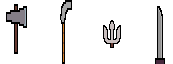
\includegraphics[width=15.5truecm]{images/weapons.png}
    \caption{A játékban megtalálható fegyverek}
    \label{fig:A játékban megtalálható fegyverek}
\end{figure}


\subsection{Ellenségek, szörnyek}

 Az ellenségek a játékban a küldetések után talán a legfontosabb mechanikái a játéknak, mert a velük való harc kiemelt szerepet kap a történet során.
Az Enemy osztálynak is az Entity a szülő osztálya, ez biztosítja, hogy mozoghassanak a szörnyek. Szerettem volna, hogy az ellenségeket különböző tulajdonságokkal tudjam felruházni, de mégis egységesen tudjam kezelni. Például a sebesség, életerő, támadási sebesség, támadások hangjai. Ezeket a tulajdonságokat a settings statikus osztály monster\_data dictionary-jében tárolom és olvasom be. És a szörnyek típúsa alapján ezeket a tulajdonságokat beállítom az adott szörny példányosításakor.

Három különböző státusszal rendelkezhet egy ellenség. A játékos karaktere, ha nincs az érzékelési sugarán belül, akkor pedig nyugalmi státuszt kap. Mozgás státuszt kap, ha a játékos karaktere a szörny érzékelési sugarán belül van, de még nem támadási sugáron belül.  Illetve támadási státuszt kap, ha támadási sugáron belül tartózkodik a játékos karaktere, ilyenkor sebzést tud bevinni a játékos karakterének és lejátsza a hozzá tartozó támadási animációt. Fontos, hogy csak bizonyos idő elteltével támadhat újra elkerülve a hirtelen túl sok sebzés bevitelét. Ezek a státuszok határozzák meg a szörnyek viselkedését és a megjelenített grafikát is a játék során.

A szörnyek mozgását úgy valósítottam meg, hogy ha a játékos egy adott sugáron belül ér a szörnyhöz képest,
 ez az úgynevezett érzékelési sugár, akkor meghatározom a játékos távolságát, 
 és ha a távolság nagyobb, mint 0, azaz nem egy helyen állnak, akkor meghatározom az irányt a két entitás vektorainak különbségének normalizálásával.
  A távolság meghatározása azért fontos, hogy megállíptsam mikor ér a játékos karaktere a szörnyhöz támadási távolságon belülre.
  Az irány értéket pedig a entitások mozgatásáért felelős move metódusnak adom át paraméterként. (Lásd \ref{subsec:Entitások})



\subsection{Zsákmányolás}
 A zsákmányolás funkciót azért tartottam fontosnak, mert plusz motivációt nyújt a játékosnak legyőzni a szörnyeket, ha szerezhet tőlük különböző erőforrásokat. Egyenlőre a szörnyek kettő különböző erőforrás hátrahagyására képesek. Tapasztalati pont bogyókat hagynak hátra, amelyek előre meghatározott mennyiségű tapasztalati pontot tartalmaznak, mindegyik szörny ilyet hagy hátra a legyőzése után. Ezenkívül aranyat is hagyhatnak hátra, két különböző fajtát, bár erre már nem minden szörny képes, és ez ritkábban fordul elő. Az egyik fajta kis mennyiségű aranyat tartalmaz, míg a másik nagyobb mennyiségű aranyat ad. 

A drop\_loot függvényt a szörnyek példányosításkor paraméterként megkapják, és ha elfogy az életpontjuk akkor hívják meg azt.
 Ez a metódus meghatároz a szörny legutóbbi pozíciójához viszonyítva egy 100x100-as négyzeten belüli pozíciót,
  ahova a zsákmányolható erőforrások fognak kirajzolásra kerülni.
   Ezt követően a szörny típusához tartozó loots listár kiolvassa a Settings osztály monster\_data dictionary-jéből,
    hogy az adott szörny milyen zsákmányokat, milyen eséllyel hagy hátra.
     Majd az előre meghatározott esély alapján véletlenszám-generálással eldönti,
      hogy milyen zsákmányokat hoz létre. A létrehozás úgy történik,
       hogy hozzá fűzi a Loot osztály egy példányát, amely tartalmazza tárgy nevét, mértékét, és helyét,  az adott pálya (World, Dungeon) példánynak a loots osztályváltozójához ami egy alapértelmezetten üres lista. 

A kirajzolása a felvehető tárgyaknak a visible sprite csoport frissítésével történik,
 mert a Loots osztály, ahogy a többi megjelenítendő objektum is, a pygame.sprite.Sprite osztályból származik le. (Lásd \ref{fig:Zsákmányolás funkció} ábra)

Tárgyak felvétele a tárgy pozíciója és a játékos karakterének távolságát vizsgálva történik,
 ha elég közel megy a játékos a tárgyhoz, akkor kitörli a loots listából a felvett tárgyat, majd az értékeit hozzáadja
  a játékos karakterének a tulajdonságaiban tárolt értékekhez.
   A hátrahagyott erőforrások addig a földön maradnak ameddig a játékos fel nem veszi azokat.
    Ez a jelenlegi játékméretnél még nem okoz teljesítménybeli romlást. 

\begin{figure}[H]
    \centering
    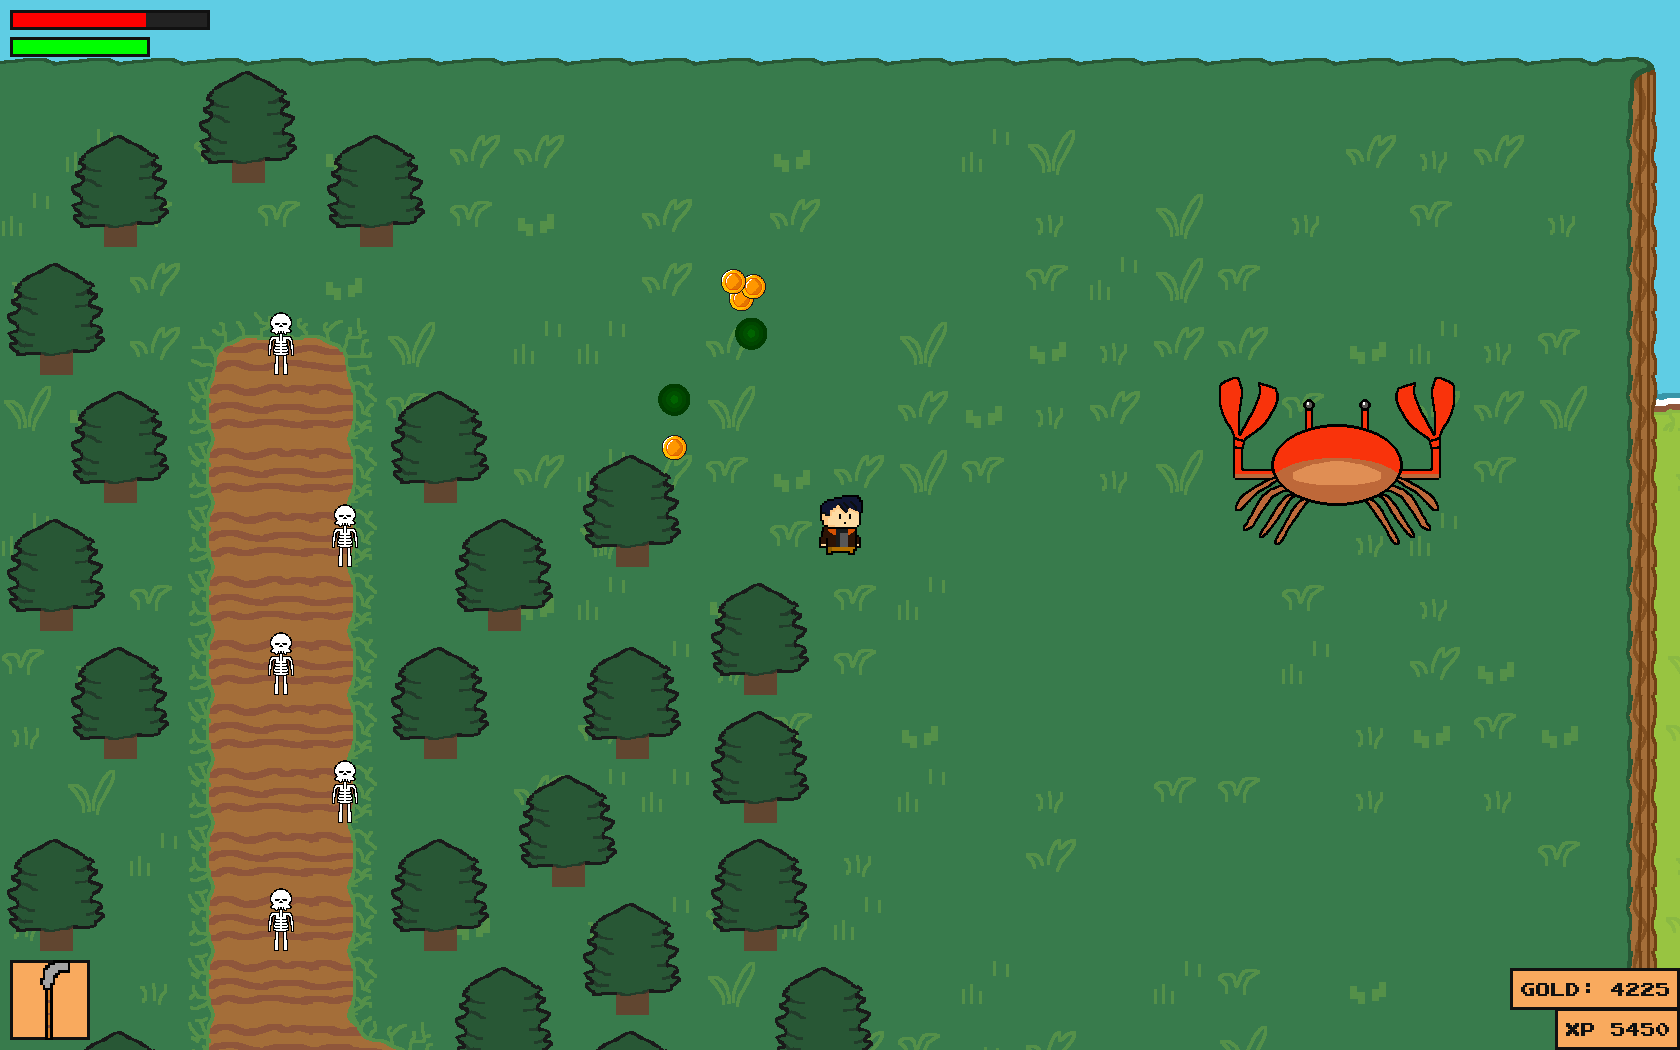
\includegraphics[width=14truecm]{images/loots.png}
    \caption{Zsákmányolás funkció}
    \label{fig:Zsákmányolás funkció}
\end{figure}

\subsection{Nem a játékos álltal vezértelt karakterek}
 Nem játékos által vezértelt karakterek, azaz NPC-k egy kalandjáték során elengedhetetlen részei a történetnek és a játékmenetnek. A szörnyek sem a játékos által vezérelt karakterek, de a játékokban az NPC megjelölést általában az egyéb, békés szerepet betöltő karaktereket hívjuk. Ahogy az szörnyek és a játékos is az Entity osztályból származik le úgy az NPC is, mert adott esetben szükség lehet mozgatásra és ütközés érzékelésre. Azonban a legtöbb esetben a játékos karaktere nem tudja megölni ezeket az entitásokat, mert a történet során szükség van rájuk. Ezért a játékos karaktere nem tud ütközni velük, és a szörnyekkel ellentétben nem tudnak támadni.


\subsection{Küldetést adó karakterek}

 A játékom egyik legfontosabb mechanikája a küldetés rendszer, mert ezen alapszik az előrehaladás, illetve a challange játékmódnál az újraindítás is a küldetések teljesítését érzékelve valósul meg. 

A Questgiver NPC (küldetést adó karakter) típust a World osztályban példányosítom, (Lásd \ref{subsec:Világ és barlangok}) és
 a példányok osztályváltozóinak inicializálásakor olvassa be a saját id-jéhez tartozó küldetéseket a Settings osztály npc\_data dictionary-jéből.
  Majd ezt követően a World osztály létrehoz a Player osztályból is egy példányt,
   amely egészen a LevelHandler osztálytól (amit már korábban említettem \ref{subsec:Pálya kezelése}) kap
    paraméterként egy questgivers\_quest\_setup függvényt amely egy trigger (aktiváló esemény) után vizsgálja,
     hogy a játékos álltal már teljesített küldetés szerepel\-e még Questgivernél. Igaz visszatérési érték esetén kitörli azt,
      ezáltal elkerülhető a küldetés ismétlődése. 
       \begin{figure}[H]
        \centering
        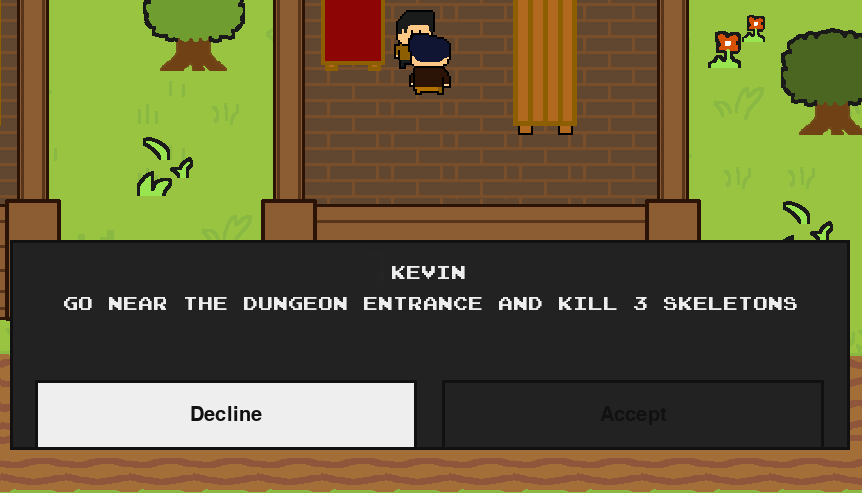
\includegraphics[width=12.0truecm]{images/dialogue.png}
        \caption{Dialógus}
        \label{fig:Dialógus rendszer}
    \end{figure}
    
Az questgiver típusú NPC-k képesek egy előre megírt dialógus megjelenítésére (Lásd \ref{fig:Dialógus rendszer} ábra), amelyben a játékos választhat két lehetőség közül, amelyek a küldetés elfogadása vagy elutasítása. A választás megerősítése történhet a kurzornak a gomb felé mozgatásával, ezután egy kattintással, vagy a billentyűzet segítségével egyaránt. A dialógus ablak megnyitásához szükséges a játékos karakteréhez viszonyított távolság érzékelése, mert egy beszélgetés során közel kell állni a kommunikációban résztvevő többi szereplőhöz, ezt hasonló módon vizsgálom, mint ahogy a szörnyek esetében az érzékelési távolságot vizsgáltam. Illetve dialógus megjelenítéséhez még szükséges, hogy az adott NPC rendelkezzen a soron következő küldetés azonosítójával is. Küldetést nem lehet kihagyni, mindegyiket sorban kell teljesíteni,
ahogy a történet halad előre. Elutasítás esetén a küldetés nem törlődik, csak a dialógus ablak bezáródik, a játékban a linearitása miatt nem lehet tovább haladni.



\subsection{Kereskedő karakter}

 Egy kalandjátékban az előrehaladás mellett fontos, hogy a nehezen megszerzett tárgyakkal,
 esetünkben az arannyal lehessen mit kezdeni, ezért egy Merchant NPC (kereskedő karakter) típus létrehozását láttam a legjobb ötletnek,
  mert rengeteg különböző módon fel lehet őket használni. 

Egyenlőre csak bájital árusításra szolgáló merchant van a játékban (élet visszatöltő, energiát növelő, sebzést növelő bájitalok árusítására szolgál).
   Ahogyan a Questgivernél, itt is a távolságvizsgálat alapján és egy gomb lenyomására történik a vásárlásra szolgáló ablak megjelenítése (Lásd \ref{fig:Merchant} ábra).
     A vásárlás során a játékos karakterének az egyenlege/arany mennyisége csökken, és a vásárolt tárgyak a hátizsákjába kerülnek.

Azt, hogy milyen tárgyakat adhat el egy bizonyos merchant, azt a Settings osztályból egy dictionary-ben tárolt azonosítók beolvasása befolyásolja.
 Illetve a Settings osztály tartalmaz egy Items dictionary-t is, amelyben a tárgyakra vonatkozó adatokat tárolom.
  Ilyen adatok például a tárgy neve, típusa, ára, hatása és annak mértéke (Például mennyi plusz erő-t ad a tárgy),
   és időtartama és a grafikának az elérési útvonala.  

\begin{figure}[H]
    \centering
    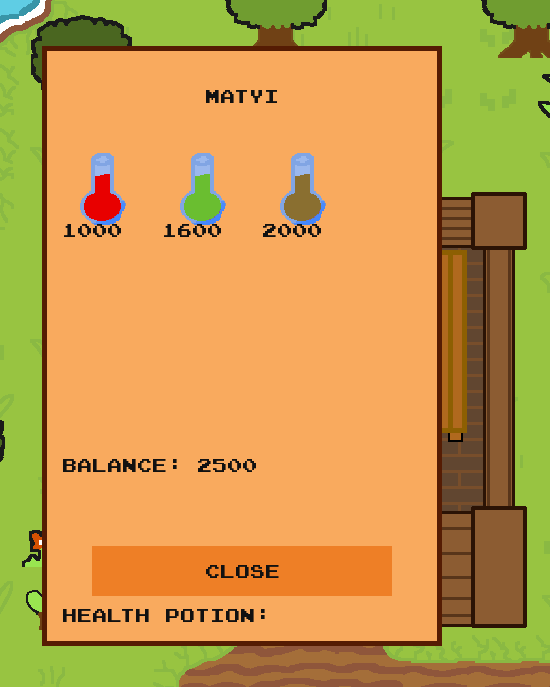
\includegraphics[width=9.0truecm]{images/merchant.png}
    \caption{Kereskedő karakter}
    \label{fig:Merchant}
\end{figure}


\subsection{Táska rendszer}

 A Quickslot azaz táska rendszer, fontos szerepet kap a játék folyamán, mert a merchanttól megvásárolt tárgyak ebbe a táskába kerülnek bele. A játékos ezeket tudja felhasználni amikor szükségét érzi, akár harc közben is.

Öt szabad férőhellyel rendelkezik a táska, ezért jól meg kell válogatni, melyek azok a fontos tárgyak, amelyeket oda szeretne helyezni a játékos. Első nekifutásra egy futószalag szerű működést képzeltem el a táska rendszernek, amelyet azért gondoltam jó ötletnek, mert a megvalósítása egyszerű volt, mert megszerzett tárgyak időrendben kerültek bele a táskába. Viszont felmerült a probléma, hogy ha más sorrendben esik kézre a felhasználónak, vagy nincs helye, akkor mit tud tenni. Ezért úgy döntöttem, hogy jobb megoldás lenne, ha az azonos tárgyakkat össze lehetne húzni egy férőhelyre, ezáltal kényelmesebbé válna a használata a táskának. Megtartottam a futószalag szerű megoldást, viszont kiegészült a tárgy összevonással, amelyet egy számláló bevezetésével oldottam meg, amely jelzi a felhasználónak, hogy még mennyi található nála abból az adott tárgy típúsból. (Lásd \ref{fig:Táska rendszer} ábra)

\begin{figure}[H]
    \centering
    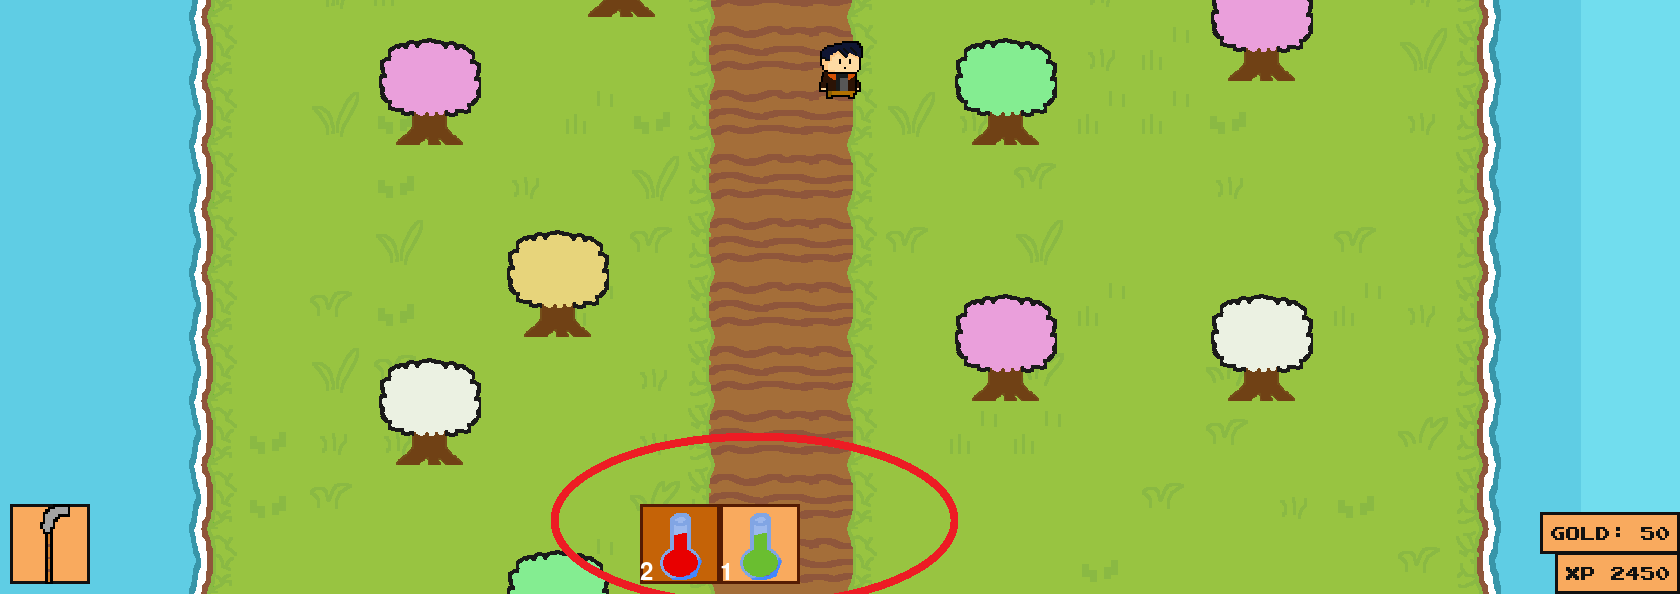
\includegraphics[width=15.5truecm]{images/inventory.png}
    \caption{Táska rendszer}
    \label{fig:Táska rendszer}
\end{figure}


\section{Adatbázis használata a programban}

 Az online mentés kezeléséhez, illetve a játékban való regisztrációhoz és bejelentkezéshez szükség volt egy backend megvalósítására, azaz egy alkalmazásra, amely kommunikációt végez a MySQL \cite{mysql} adatbázissal. Az adatbázis struktúrát a MySQL Workbench \cite{mysql-workbench} asztali alkalmazásban építettem fel, eddig az általam használt alkalmazások küzül ez volt ami felhasználóbarát módon volt megvalósítva.  A kommunikációt a FastAPI \cite{fastapi} nevű python könyvtár segítségével valósítottam meg. A FastAPI egy modern, gyors, könnyű keretrendszer a microservice-ekhez talán a legjobb választás python programozási nyelv esetében.

Az adatokat különböző requestek és a megfelelő endpointok segítségével tudjuk elérni, vagy adott esetben felvinni, frissíteni.
 A FastAPI érzékeli, hogy egy kérés érkezett a rendszerbe, és ha az adott kérés teljesíthető,
  akkor az esetemben megkezdi a kommunikációt a mysql adatbázissal és a visszakapott adatokat BaseModell \cite{basemodell} típusú objektumokba tölti,
   amelyekek a Pydantic \cite{pydantic} könyvtárnak köszönhetőek. Ez a modell azért fontos, mert validálja,
    hogy a kérésben szereplő adatok megfelelnek-e a megadott adatstruktúrának.
     Miután a validálás is sikeresen lezajlott, a FastAPI visszaküldi a végpont kérésre a megfelelő választ.


\chapter{Továbbfejlesztési lehetőségek}




\section{Táska rendszer}
több item lesz kell több hely, és lehessen sortolni

\section{Ellenségek}
Több ellenség, egyedi képességekkel (most mind egyként működik)







A fejezetben be kell mutatni, hogy az elkészült alkalmazás hogyan használható.
(Az, hogy hogyan kell, hogy működjön, és hogy hogy lett elkészítve, az előző fejezetekben már megtörtént.)

Jellemzően az alábbi dolgok kerülhetnek ide.
\begin{itemize}
\item Tesztfuttatások. Le lehet írni a futási időket, memória és tárigényt.
\item Felhasználói kézikönyv jellegű leírás. Kifejezetten a végfelhasználó szempontjából lehet azt bemutatni, hogy mit hogy lehet majd használni.
\item Kutatás kapcsán ide főként táblázatok, görbék és egyéb részletes összesítések kerülhetnek.
\end{itemize}

\chapter{Összefoglalás}

Hasonló szerepe van, mint a bevezetésnek.
Itt már múltidőben lehet beszélni.
A szerző saját meglátása szerint kell összegezni és értékelni a dolgozat fontosabb eredményeit.
Meg lehet benne említeni, hogy mi az ami jobban, mi az ami kevésbé jobban sikerült a tervezettnél.
El lehet benne mondani, hogy milyen további tervek, fejlesztési lehetőségek vannak még a témával kapcsolatban.


%biblatex verzió
%a bibintoc heading stílussal megjelenik a tartalomjegyzékben, title-lel a megjelenő címsor szövege módosítható
\printbibliography[heading=bibintoc,%
title=Források]
%sima bibtex verzió
%\bibliographystyle{plain}
%\bibliography{dolgozat.bib}

\pagestyle{empty}

\section*{CD Használati útmutató}

Ennek a címe lehet például \textit{A mellékelt CD tartalma} vagy \textit{Adathordozó használati útmutató} is.

Ez jellemzően csak egy fél-egy oldalas leírás.
Arra szolgál, hogy ha valaki kézhez kapja a szakdolgozathoz tartozó CD-t, akkor tudja, hogy mi hol van rajta.
Jellemzően elég csak felsorolni, hogy milyen jegyzékek vannak, és azokban mi található.
Az elkészített programok telepítéséhez, futtatásához tartozó instrukciók kerülhetnek ide.

A CD lemezre mindenképpen rá kell tenni
\begin{itemize}
\item a dolgozatot egy \texttt{dolgozat.pdf} fájl formájában,
\item a LaTeX forráskódját a dolgozatnak,
\item az elkészített programot, fontosabb futási eredményeket (például ha kép a kimenet),
\item egy útmutatót a CD használatához (ami lehet ez a fejezet külön PDF-be vagy MarkDown fájlként kimentve).
\end{itemize}


\end{document}
